
\documentclass[a4paper,11pt]{article}%,twocolumn
%% packages

\usepackage{blindtext} % needed for creating dummy text passages
%\usepackage{ngerman} % needed for German default language
\usepackage{amsmath} % needed for command eqref
\usepackage{amssymb} % needed for math fonts
\usepackage[colorlinks=true,breaklinks]{hyperref} % needed for creating hyperlinks in the document, the option colorlinks=true gets rid of the awful boxes, breaklinks breaks lonkg links (list of figures), and ngerman sets everything for german as default hyperlinks language
\usepackage[hyphenbreaks]{breakurl} % ben�tigt f�r das Brechen von URLs in Literaturreferenzen, hyphenbreaks auch bei links, die �ber eine Seite gehen (mit hyphenation).
\usepackage{xcolor}
\definecolor{c1}{rgb}{0,0,1} % blue
\definecolor{c2}{rgb}{0,0.3,0.9} % light blue
\definecolor{c3}{rgb}{0.3,0,0.9} % red blue
\hypersetup{
    linkcolor={c1}, % internal links
    citecolor={c2}, % citations
    urlcolor={c3} % external links/urls
}
%\usepackage{cite} % needed for cite
\usepackage[square,authoryear]{natbib} % needed for cite and abbrvnat bibliography style
\usepackage[nottoc]{tocbibind} % needed for displaying bibliography and other in the table of contents
\usepackage{graphicx} % needed for \includegraphics 
\usepackage{longtable} % needed for long tables over pages
\usepackage{bigstrut} % needed for the command \bigstrut
\usepackage{enumerate} % needed for some options in enumerate
%\usepackage{todonotes} % needed for todos
\usepackage{makeidx} % needed for creating an index
\makeindex
\usepackage{gensymb}
\usepackage{url}
\usepackage{psfrag}
\usepackage{multirow}
\usepackage{subfigure}
%% page settings

\usepackage[top=20mm, bottom=20mm,left=15mm,right=15mm]{geometry} % needed for page border settings
\parindent=0mm % for space of first line of new text block
\sloppy % for writing with hyphenless justification (tries to)
\hyphenation{} % use hyphenation of tolerance parametershttp://www.jr-x.de/publikationen/latex/tipps/zeilenumbruch.html
\hyphenpenalty=10000
\exhyphenpenalty=10000
\usepackage{fancyhdr} % needed for head and foot options
%% my macros

%% Text fomats
\newcommand{\tbi}[1]{\textbf{\textit{#1}}}

%% Math fonts
\newcommand{\bbA}{\mathbb{A}}
\newcommand{\bbB}{\mathbb{B}}
\newcommand{\bbC}{\mathbb{C}}
\newcommand{\bbD}{\mathbb{D}}
\newcommand{\bbE}{\mathbb{E}}
\newcommand{\bbF}{\mathbb{F}}
\newcommand{\bbG}{\mathbb{G}}
\newcommand{\bbH}{\mathbb{H}}
\newcommand{\bbI}{\mathbb{I}}
\newcommand{\bbJ}{\mathbb{J}}
\newcommand{\bbK}{\mathbb{K}}
\newcommand{\bbL}{\mathbb{L}}
\newcommand{\bbM}{\mathbb{M}}
\newcommand{\bbN}{\mathbb{N}}
\newcommand{\bbO}{\mathbb{O}}
\newcommand{\bbP}{\mathbb{P}}
\newcommand{\bbQ}{\mathbb{Q}}
\newcommand{\bbR}{\mathbb{R}}
\newcommand{\bbS}{\mathbb{S}}
\newcommand{\bbT}{\mathbb{T}}
\newcommand{\bbU}{\mathbb{U}}
\newcommand{\bbV}{\mathbb{V}}
\newcommand{\bbW}{\mathbb{W}}
\newcommand{\bbX}{\mathbb{X}}
\newcommand{\bbY}{\mathbb{Y}}
\newcommand{\bbZ}{\mathbb{Z}}
\usepackage[ framed, numbered]{matlab-prettifier}%framed,%
\usepackage{listings}
\usepackage{physics}
\usepackage{pdfpages}
\usepackage[toc,page]{appendix}
\usepackage{float}
\usepackage{hyperref}

% for code
\usepackage{listings}
\usepackage{color}
% Define colors
\definecolor{codegreen}{rgb}{0,0.6,0}
\definecolor{codegray}{rgb}{0.5,0.5,0.5}
\definecolor{codepurple}{rgb}{0.58,0,0.82}
\definecolor{backcolour}{rgb}{0.95,0.95,0.92}
% Setup the listings package
\lstset{
    backgroundcolor=\color{backcolour},   
    commentstyle=\color{codegreen},
    keywordstyle=\color{magenta},
    numberstyle=\tiny\color{codegray},
    stringstyle=\color{codepurple},
    basicstyle=\footnotesize,
    breakatwhitespace=false,         
    breaklines=true,                 
    captionpos=b,                    
    keepspaces=true,                                
    showspaces=false,                
    showstringspaces=false,
    showtabs=false,                  
    tabsize=2
}

\newenvironment{qanda}{\setlength{\parindent}{0pt}}{\bigskip}
\newcommand{\Q}{\bigskip\bfseries Q: }
\newcommand{\A}{\par\textbf{Answer: } \normalfont}

\begin{document}
\begin{titlepage}
\center % Center everything on the page

%-------------------------------------------------------------------------------------
%	HEADING SECTIONS
%------------------------------------------------------------------------------------
\textbf{\large Department of Electrical and Computer Engineering}\\[0.5cm]
\textbf{\Large University of Colorado at Boulder}\\[1cm]
\textbf{\large ECEN5623 - Real Time Embedded Systems }\\[2cm]

\includegraphics[width=0.3\textwidth]{figures/cu}\\[2cm]

	
%-------------------------------------------------------------------------------------
%	TITLE SECTION
%------------------------------------------------------------------------------------
\textbf{\Huge Exercise 5 }\\[0.2cm]



%----------------------------------------------------------------------------------------
%	MEMBERS SECTION
%----------------------------------------------------------------------------------------


\vfill

\textbf{\large Submitted by}\\[0.5cm]

{\large Parth | Jithedra}\\[0.5cm]	

%----------------------------------------------------------------------------------------
%	DATE SECTION
%----------------------------------------------------------------------------------------

\textbf{\large Submitted on}
\textbf{\Large \today} % Date, change the \today to a set date if you want to be precise

%----------------------------------------------------------------------------------------

\vfill % Fill the rest of the page with whitespace

\end{titlepage}


\pagebreak

\tableofcontents
\listoffigures
\listoftables
\vfill
\begin{center}
	\textbf{\textit{*PDF is clickable}}
\end{center}

\pagebreak

\section*{Objective}
\begin{enumerate}
	\item Understand the provided seqgen.c and seqgen2x.c code, which emulates a cyclic executive real-time system with multiple services running at separate frequencies.
	
	\item Build and execute the provided code on different platforms (Linux on DE1-SoC, Raspberry Pi, or Jetson board) and determine the worst-case execution time (WCET) for each service. Create a rate-monotonic (RM) schedule in Cheddar using the WCET estimates and calculate the CPU utilization.

\end{enumerate}

\pagebreak
\begin{qanda}
	\section{Question 1}
	\begin{enumerate}
		\item[] \Q [20 points] Download seqgen.c and seqgen2x.c (or unzip them from the provided zip file for
			this exercise) and build them in Linux on the Altera DE1-SOC, Raspberry Pi or Jetson board
			and execute the code. Describe what it is doing and make sure you understand how to use it
			to structure an embedded system. Determine the worst case execution time (WCET) for each
			service by printing or logging timestamps between two points in your code or by use of a
			profiling tool. Determine D, T, and C for each service and create an RM schedule in
			Cheddar using your WCET estimates. Calculate the \% CPU utilization for this system.
			\A

			\subsection{API Explanation:}
			\begin{enumerate}
				\item pthread\_create(): This function is used to create a new thread. It takes four arguments: a pointer to the thread identifier, a pointer to the thread attributes, the thread function, and a pointer to the thread arguments. In this code, it is used to create the Sequencer thread and the seven Service threads.
				\item pthread\_join(): This function is used to wait for the termination of a thread. It takes two arguments: the thread identifier and a pointer to the return value. In this code, it is used to wait for the termination of all the created threads.
				\item sem\_init(): This function is used to initialize an unnamed semaphore. It takes three arguments: a pointer to the semaphore object, a flag indicating whether the semaphore is shared between processes, and the initial value of the semaphore. In this code, it is used to initialize the semaphores for each Service thread.
				\item sem\_wait(): This function is used to decrement (lock) a semaphore. If the semaphore's value is greater than zero, the decrement proceeds, and the function returns immediately. If the semaphore's value is zero, the call blocks until it becomes possible to perform the decrement. In this code, it is used by the Service threads to wait for their respective semaphores to be released by the Sequencer thread.
				\item sem\_post(): This function is used to increment (unlock) a semaphore. If the semaphore's value consequently becomes greater than zero, then another process or thread blocked in a sem\_wait() call will be woken up and proceed to lock the semaphore. In this code, it is used by the Sequencer thread to release the semaphores for each Service thread based on their respective rates.
				\item clock\_gettime(): This function is used to retrieve the current time of the specified clock. It takes two arguments: the clock ID and a pointer to a timespec structure to store the retrieved time. In this code, it is used in the getTimeMsec() function to retrieve the current time in milliseconds using the CLOCK\_MONOTONIC clock.
				\item sched\_setscheduler(): This function is used to set the scheduling policy and parameters for a thread. It takes three arguments: the thread identifier, the scheduling policy, and a pointer to the scheduling parameters. In this code, it is used to set the scheduling policy of the main thread to SCHED\_FIFO with the maximum priority.
			\end{enumerate}







			\subsection{Code Flow:}
			The code follows a sequencer-based design pattern, where a high-priority Sequencer thread releases semaphores for each Service thread at specific rates. The main steps in the code flow are as follows:
			\begin{enumerate}
				\item The main thread is created with the highest priority using the SCHED\_FIFO scheduling policy.
				\item Semaphores are initialized for each Service thread using sem\_init().
				\item The Service threads (Service\_1 to Service\_7) are created using pthread\_create() with specific attributes and priorities.
				\item The Sequencer thread is created using pthread\_create() with the highest priority.
				\item The Sequencer thread runs in a loop, releasing semaphores for each Service thread at their respective rates based on the sequencer count.
				\item Each Service thread waits for its respective semaphore using sem\_wait() and then performs its specific task.
				\item The Sequencer thread continues to run until a specified number of periods have elapsed or an abort flag is set.
				\item Once the Sequencer thread completes, it releases all the semaphores and sets abort flags for each Service thread.
				\item The main thread waits for all the created threads to terminate using pthread\_join().
			\end{enumerate}

			\textbf{Initialization Calibration:}
			The code begins with an initialization phase where the execution time of a specific workload is measured. This calibration is performed to determine the baseline execution time without any interference from other tasks. The workload consists of 10 iterations of a computationally intensive task, and the execution time for each iteration is recorded.

			Here's an example of the calibration output:
			\begin{lstlisting}
Apr  9 09:10:45 iteration (0) Start time: 1712675444993.189941 ms , 
end time: 1712675445083.585938 ms , execution time: 90.395996 ms

Apr  9 09:10:45 iteration (1) Start time: 1712675445083.662109 ms , 
end time: 1712675445169.305908 ms , execution time: 85.643799 ms
...
Apr  9 09:10:45 iteration (9) Start time: 1712675445756.726074 ms , 
end time: 1712675445840.318115 ms , execution time: 83.592041 ms

Apr  9 09:10:45 ***** Average time 84.656934 *****
\end{lstlisting}

			The calibration shows that the average execution time of the workload is around 84.66 milliseconds, with some variations between iterations.


			\subsection{Output Analysis:}
			After the system runs for a specified duration, the code provides an output analysis that summarizes the execution characteristics of each task. The analysis includes the worst-case execution time (WCET), total execution time, number of execution cycles, and average execution time for each task.\\

			Here's an example of the output analysis:
			\begin{lstlisting}
Apr  9 09:11:15 **** Task (1):  WCET: 92.489014, total_execution time : 7542.553467,
 execution cycles : 89, average execution time : 84.747792 ****

Apr  9 09:11:15 **** Task (2):  WCET: 85.020996, total_execution time : 2430.170898,
 execution cycles : 29, average execution time : 83.798996 ****
...
Apr  9 09:11:15 **** Task (7):  WCET: 168.037109, total_execution time : 335.905273,
execution cycles : 2, average execution time : 167.952637 ****
\end{lstlisting}

			The analysis provides insights into the timing behavior of each task. For example, Task 1 has a WCET of 92.49 milliseconds, a total execution time of 7542.55 milliseconds across 89 execution cycles, and an average execution time of 84.75 milliseconds.

			\textbf{Preemption and Critical Instant:}
			The code execution involves multiple tasks running concurrently with different priorities. When a higher-priority task is released, it can preempt the execution of a lower-priority task. The point at which all tasks are released simultaneously is known as the critical instant, which represents the worst-case scenario for task execution.

			In the provided logs, we can observe instances of preemption and the critical instant. For example:

			\begin{lstlisting}
Apr  9 09:11:15 Task 1, Frame Sampler start 90 @ msec=1712675475936.939941
Apr  9 09:11:16 Task 1, Frame Sampler Execution complete @ msec=1712675476020.899902,
 execution time : 83.959961 ms

Apr  9 09:11:16 Task 2, Time-stamp with Image Analysis
 thread start 30 @ msec=1712675476020.974121

Apr  9 09:11:16 Task 2, Time-stamp with Image Analysis
 thread Execution complete @ msec=1712675476104.347900, execution time : 83.373779 ms

Apr  9 09:11:16 Task 4, Time-stamp Image Save to File
 start 30 @ msec=1712675476104.416016

Apr  9 09:11:16 Task 4, Time-stamp Image Save to File
 Execution complete @ msec=1712675476188.677002, execution time : 84.260986 ms

Apr  9 09:11:16 Task 6, Send Time-stamped Image to Remote
 start 30 @ msec=1712675476188.757080
\end{lstlisting}

			In this snippet, we can see that Task 1 starts executing and completes its execution. Immediately after Task 1 completes, Task 2 starts executing, followed by Task 4 and Task 6. This sequence demonstrates the preemption of lower-priority tasks by higher-priority tasks.

			\textbf{Execution Time Variations and Interference:}
			The execution time of tasks can vary due to interference from other tasks running concurrently on the system. When multiple tasks compete for shared resources, such as CPU time or memory, it can lead to delays and increased execution times.\\

			In the output analysis, we can observe variations in the execution time of tasks. For example, Task 6 has a relatively high WCET of 177.17 milliseconds compared to its average execution time of 168.94 milliseconds. This difference can be attributed to interference from other tasks during the worst-case scenario.\\

			Similarly, the logs show variations in execution time for the same task across different instances. For example:

			\begin{lstlisting}
Apr  9 09:11:15 Task 1, Frame Sampler start 89 @ msec=1712675475600.466064
Apr  9 09:11:15 Task 1, Frame Sampler Execution 
complete @ msec=1712675475684.990967, execution time : 84.524902 ms
...
Apr  9 09:11:15 Task 1, Frame Sampler start 90 @ msec=1712675475936.939941
Apr  9 09:11:16 Task 1, Frame Sampler Execution 
complete @ msec=1712675476020.899902, execution time : 83.959961 ms
\end{lstlisting}
			Here, we can see that Task 1 has an execution time of 84.52 milliseconds in one instance and 83.96 milliseconds in another instance. These variations can be caused by interference from other tasks executing concurrently.

			\textbf{Critical Instant and Worst-Case Execution Time:}
			The critical instant occurs when all tasks are released simultaneously, leading to the worst-case execution time for each task. In the provided logs, we can identify the critical instant when multiple tasks start executing in quick succession.

			For example:

			\begin{lstlisting}
Apr  9 09:11:15 Task 1, Frame Sampler start 90 @ msec=1712675475936.939941
Apr  9 09:11:16 Task 1, Frame Sampler Execution
complete @ msec=1712675476020.899902, execution time : 83.959961 ms


Apr  9 09:11:16 Task 2, Time-stamp with Image Analysis 
thread start 30 @ msec=1712675476020.974121

Apr  9 09:11:16 Task 2, Time-stamp with Image Analysis
thread Execution complete @ msec=1712675476104.347900, execution time : 83.373779 ms


Apr  9 09:11:16 Task 4, Time-stamp Image Save to File s
tart 30 @ msec=1712675476104.416016

Apr  9 09:11:16 Task 4, Time-stamp Image Save to File 
Execution complete @ msec=1712675476188.677002, execution time : 84.260986 ms


Apr  9 09:11:16 Task 6, Send Time-stamped Image to Remote 
start 30 @ msec=1712675476188.757080

Apr  9 09:11:16 Task 6, Send Time-stamped Image to
Remote Execution complete @ msec=1712675476272.794922, execution time : 84.037842 ms
\end{lstlisting}

			In this scenario, Tasks 1, 2, 4, and 6 start executing in close proximity, representing a critical instant. The execution times of these tasks in this critical instant are likely to be closer to their WCET values due to the increased interference and resource contention.\\

			Overall, the initialization calibration provides a baseline for execution time, while the output analysis and logs help identify preemption, critical instants, and variations in execution time caused by interference. By examining these factors, developers can assess the timing behavior and predictability of the system under different scenarios and make necessary optimizations to ensure the desired real-time performance.\\


			In summary, the sequencer is running at 60 Hz, and the other tasks are running at their defined frequencies as specified in the code comments:\\
			\begin{enumerate}
				\item Task 1: 30 Hz
				\item Task 2: 10 Hz
				\item Task 3: 5 Hz
				\item Task 4: 10 Hz
				\item Task 5: 5 Hz
				\item Task 6: 10 Hz
				\item Task 7: 1 Hz
			\end{enumerate}





			To confirm the sequencer and task frequencies from the code output, let's analyze the relevant log messages.

			\textbf{Sequencer frequency:}
			The sequencer logs a message at the beginning of each cycle, including the cycle count and timestamp. By calculating the time difference between consecutive cycles, we can determine the sequencer frequency.

			For example:

			\begin{lstlisting}
Apr  9 09:10:45 Sequencer cycle 1 @ sec=0, msec=875
Apr  9 09:10:45 Sequencer cycle 2 @ sec=0, msec=908
Apr  9 09:10:45 Sequencer cycle 3 @ sec=0, msec=942
Apr  9 09:10:45 Sequencer cycle 4 @ sec=0, msec=975
\end{lstlisting}

			The time difference between cycles is consistently around 33-34 milliseconds, which corresponds to a frequency of approximately 30 Hz (1000 ms / 33.33 ms = 30 Hz).

			\textbf{Task frequencies:}
			Each task's release is logged with a message indicating the task name and release count. By observing the release patterns, we can confirm the task frequencies.
			\begin{enumerate}
				\item Task 1 (Frame Sampler thread):

				      \begin{lstlisting}
Apr  9 09:10:46 Task 1 (Frame Sampler thread) Released
Apr  9 09:10:46 Task 1 (Frame Sampler thread) Released
Apr  9 09:10:46 Task 1 (Frame Sampler thread) Released
Apr  9 09:10:47 Task 1 (Frame Sampler thread) Released
				\end{lstlisting}

				      Task 1 is released every 2 sequencer cycles, corresponding to a frequency of 15 Hz (30 Hz / 2).
				\item Task 2 (Time-stamp with Image Analysis thread) and Task 4 (Time-stamp Image Save to File thread):

				      \begin{lstlisting}
Apr  9 09:10:46 Task 2 (Time-stamp with Image Analysis thread) Released
Apr  9 09:10:46 Task 4 (Time-stamp Image Save to File thread) Released
Apr  9 09:10:47 Task 2 (Time-stamp with Image Analysis thread) Released
Apr  9 09:10:47 Task 4 (Time-stamp Image Save to File thread) Released
				\end{lstlisting}

				      Tasks 2 and 4 are released every 6 sequencer cycles, corresponding to a frequency of 5 Hz (30 Hz / 6).
				\item Task 3 (Difference Image Proc thread) and Task 5 (Processed Image Save to File thread):


				      \begin{lstlisting}
Apr  9 09:10:48 Task 3 ( Difference Image Proc thread) Released
Apr  9 09:10:48 Task 5 (Processed Image Save to File thread) Released
Apr  9 09:10:49 Task 3 ( Difference Image Proc thread) Released
Apr  9 09:10:49 Task 5 (Processed Image Save to File thread) Released
				\end{lstlisting}

				      Tasks 3 and 5 are released every 12 sequencer cycles, corresponding to a frequency of 2.5 Hz (30 Hz / 12).
				\item Task 6 (Send Time-stamped Image to Remote thread):

				      \begin{lstlisting}
Apr  9 09:10:46 Task 6 (Send Time-stamped Image to Remote thread) Released
Apr  9 09:10:47 Task 6 (Send Time-stamped Image to Remote thread) Released
Apr  9 09:10:48 Task 6 (Send Time-stamped Image to Remote thread) Released
				\end{lstlisting}

				      Task 6 is released every 6 sequencer cycles, corresponding to a frequency of 5 Hz (30 Hz / 6).
				\item Task 7 (10 sec Tick Debug thread):


				      Copy code
				      \begin{lstlisting}
Apr  9 09:10:55 Task 7 (10 sec Tick Debug thread) Released
Apr  9 09:11:05 Task 7 (10 sec Tick Debug thread) Released
\end{lstlisting}

				      Task 7 is released every 60 sequencer cycles, corresponding to a frequency of 0.5 Hz (30 Hz / 60).


			\end{enumerate}






			Based on the output analysis, we can confirm that the sequencer is running at approximately 30 Hz, and the tasks are released at their specified frequencies relative to the sequencer cycles.


			\textbf{Let's examine the output to identify instances of jitter:}

			Task release jitter: If we look at the timestamps of consecutive task releases, we can see if there are any significant variations from the expected release times. For example, let's consider Task 1 (Frame Sampler thread) releases:

			\begin{lstlisting}
Apr  9 09:10:46 Task 1 (Frame Sampler thread) Released
Apr  9 09:10:46 Task 1 (Frame Sampler thread) Released
Apr  9 09:10:47 Task 1 (Frame Sampler thread) Released
Apr  9 09:10:47 Task 1 (Frame Sampler thread) Released
\end{lstlisting}

			Ideally, Task 1 should be released every 2 sequencer cycles (approximately 66.67 ms apart). However, the actual release timestamps may vary slightly from the expected times, indicating the presence of release jitter.
			Task completion jitter: By comparing the completion timestamps of a task across different instances, we can identify any variations in the task's execution time, which contributes to completion jitter. For instance, let's analyze the completion times of Task 1:


			\begin{lstlisting}
Apr  9 09:10:46 Task 1, Frame Sampler Execution 
complete @ msec=1712675446261.259033, execution time : 84.063965 ms

Apr  9 09:10:46 Task 1, Frame Sampler Execution 
complete @ msec=1712675446604.060059, execution time : 92.489014 ms

Apr  9 09:10:47 Task 1, Frame Sampler Execution 
complete @ msec=1712675446929.551025, execution time : 83.798096 ms

Apr  9 09:10:47 Task 1, Frame Sampler Execution 
complete @ msec=1712675447264.642090, execution time : 85.116211 ms
\end{lstlisting}
			The execution times of Task 1 vary between different instances, ranging from around 83.8 ms to 92.5 ms. This variation in execution time contributes to completion jitter.
			Sequencer jitter: The sequencer itself may experience jitter, which can propagate to the task releases. If the sequencer cycles are not precisely periodic, it can introduce jitter in the task release times. We can analyze the sequencer cycle timestamps to identify any variations:

			\begin{lstlisting}
Apr  9 09:10:45 Sequencer cycle 1 @ sec=0, msec=875
Apr  9 09:10:45 Sequencer cycle 2 @ sec=0, msec=908
Apr  9 09:10:45 Sequencer cycle 3 @ sec=0, msec=942
Apr  9 09:10:45 Sequencer cycle 4 @ sec=0, msec=975
Apr  9 09:10:46 Sequencer cycle 5 @ sec=1, msec=9
\end{lstlisting}
			The time differences between consecutive sequencer cycles may vary slightly, indicating the presence of sequencer jitter.
			Jitter can be caused by various factors, such as:
			\begin{itemize}
				\item System load and resource contention
				      Interference from other tasks or processes
				      Scheduling overhead and context switching
				      Timer resolution and accuracy
				      Hardware interrupts and other system events
			\end{itemize}



			From the output, we can observe that CPU affinity is set for each task. Here are a few examples:

			Task 1 (Frame Sampler thread):


			\begin{lstlisting}
Apr  9 09:10:46 Task 1, Frame Sampler start 1 @ msec=1712675446177.195068
Apr  9 09:10:46 Task 1, Frame Sampler Execution 
complete @ msec=1712675446261.259033, execution time : 84.063965 ms

Apr  9 09:10:46 Task 1, Frame Sampler start 2 @ msec=1712675446511.571045
Apr  9 09:10:46 Task 1, Frame Sampler Execution 
complete @ msec=1712675446604.060059, execution time : 92.489014 ms
\end{lstlisting}
			Task 1 instances are executed sequentially, indicating that they are running on the same CPU core without interference from other tasks.
			Task 2 (Time-stamp with Image Analysis thread) and Task 4 (Time-stamp Image Save to File thread):


			\begin{lstlisting}
Apr  9 09:10:46 Task 2, Time-stamp with Image Analysis thread 
start 1 @ msec=1712675446929.628906

Apr  9 09:10:47 Task 2, Time-stamp with Image Analysis 
thread Execution complete @ msec=1712675447013.268066, execution time : 83.639160 ms

Apr  9 09:10:47 Task 4, Time-stamp Image Save to File 
start 1 @ msec=1712675447013.284912

Apr  9 09:10:47 Task 4, Time-stamp Image Save to File Execution 
complete @ msec=1712675447096.925049, execution time : 83.640137 ms
\end{lstlisting}
			Task 2 and Task 4 are executed sequentially, one after the other. This suggests that they are running on different CPU cores, allowing for parallel execution without contention.
			Task 3 (Difference Image Proc thread) and Task 5 (Processed Image Save to File thread):


			\begin{lstlisting}
Apr  9 09:10:48 Task 3, Difference Image Proc  
start 1 @ msec=1712675448271.108887

Apr  9 09:10:48 Task 3, Difference Image Proc 
Execution complete @ msec=1712675448356.852051, execution time : 85.743164 ms

Apr  9 09:10:48 Task 5, Processed Image Save to File 
start 1 @ msec=1712675448356.884033

Apr  9 09:10:48 Task 5, Processed Image Save to File Execution 
complete @ msec=1712675448442.035889, execution time : 85.151855 ms


			\end{lstlisting}
			Task 3 and Task 5 are executed sequentially, indicating that they are running on different CPU cores, allowing for parallel execution.
			Task 6 (Send Time-stamped Image to Remote thread):
			\begin{lstlisting}
Apr  9 09:10:47 Task 6, Send Time-stamped Image to Remote 
start 1 @ msec=1712675447096.968994

Apr  9 09:10:47 Task 6, Send Time-stamped Image to Remote 
Execution complete @ msec=1712675447267.272949, execution time : 170.303955 ms
\end{lstlisting}

			Task 6 instances are executed independently, suggesting that they are running on a dedicated CPU core.
			From the output, we can see that tasks are executed in a non-overlapping manner, with each task running to completion before the next task starts. This behavior indicates that CPU affinity is set, and parallel tasks are not running simultaneously on the same CPU core.

			\subsection{SEQGEN2x}

			The code flow and everything is same in the seqgen2 code but the frequencies of tasks is 10 times the original and I have changed load to 10ms load here is the output analysis

			\begin{lstlisting}
Apr  9 22:17:21 rog seqgen2: **** Task 1):  WCET: 13.337891, 
total_execution time : 4801.594238, execution cycles : 449, 
average execution time : 10.693974 **** #012 

Apr  9 22:17:21 rog seqgen2: **** Task 2):  WCET: 12.876953, 
total_execution time : 1578.309814, execution cycles : 149, 
average execution time : 10.592683 **** #012 

Apr  9 22:17:21 rog seqgen2: **** Task 3):  WCET: 25.176025, 
total_execution time : 966.507324, execution cycles : 74, 
average execution time : 13.060910 **** #012 

Apr  9 22:17:21 rog seqgen2: **** Task 4):  WCET: 25.923828, 
total_execution time : 2069.981689, execution cycles : 149,
average execution time : 13.892495 **** #012 

Apr  9 22:17:21 rog seqgen2: **** Task 5):  WCET: 24.409912, 
total_execution time : 1365.902832, execution cycles : 74, 
average execution time : 18.458146 **** #012 

Apr  9 22:17:21 rog seqgen2: **** Task 6):  WCET: 26.864014, 
total_execution time : 2668.886475, execution cycles : 149, 
average execution time : 17.911990 **** #012 

Apr  9 22:17:21 rog seqgen2: **** Task 7):  WCET: 68.493164, 
total_execution time : 259.799805, execution cycles : 14, 
average execution time : 18.557129 **** #012 
\end{lstlisting}


			due to faster execution and higher Interference we can see jitter in the task execution which is far higher than 10ms load that we set. This shows higher utilization in linux tends to make task more non-deterministic

			\subsection{Comparison with Linux and FreeRTOS:}
			The provided code is a Linux implementation of a real-time system using POSIX threads and semaphores. Let's compare it with a FreeRTOS implementation:
			\begin{enumerate}
				\item Threading:\\
				      In Linux, POSIX threads (pthreads) are used to create and manage threads. The pthread\_create() function is used to create threads, and pthread\_join() is used to wait for thread termination.
				      In FreeRTOS, tasks are used instead of threads. The xTaskCreate() function is used to create tasks, and the vTaskDelete() function is used to delete tasks.
				\item Synchronization:\\
				      In Linux, POSIX semaphores (sem\_t) are used for synchronization between threads. The sem\_init(), sem\_wait(), and sem\_post() functions are used to initialize, wait, and post semaphores, respectively.
				      In FreeRTOS, binary semaphores (SemaphoreHandle\_t) and counting semaphores are used for synchronization between tasks. The xSemaphoreCreateBinary() function is used to create binary semaphores, and the xSemaphoreTake() and xSemaphoreGive() functions are used to take and give semaphores, respectively.
				\item Scheduling:\\
				      In Linux, the SCHED\_FIFO scheduling policy is used to achieve real-time behavior. The sched\_setscheduler() function is used to set the scheduling policy and priority of threads.
				      In FreeRTOS, the task scheduler is used to manage task execution based on their priorities. The vTaskPrioritySet() function is used to set the priority of tasks.
				\item Timing:
				      In Linux, the clock\_gettime() function is used to retrieve the current time with nanosecond resolution. The CLOCK\_MONOTONIC clock is used to avoid any time adjustments.
				      In FreeRTOS, the xTaskGetTickCount() function is used to retrieve the current tick count, which represents the number of ticks since the scheduler started. The portTICK\_PERIOD\_MS constant is used to convert ticks to milliseconds.
				\item Preemption:
				      In Linux, preemption is enabled by default, allowing higher-priority threads to preempt lower-priority threads.
				      In FreeRTOS, preemption can be enabled or disabled using the configUSE\_PREEMPTION configuration flag. When enabled, higher-priority tasks can preempt lower-priority tasks.
				\item Timestamps and WCET Estimates:
				      The code includes timestamp logging using the syslog() function to record the start and completion times of each Service thread. These timestamps can be used to estimate the execution times of each thread.
			\end{enumerate}








			To determine the worst-case execution time (WCET) for each Service thread, you would need to analyze the execution times over multiple runs and consider the longest observed execution time as the WCET estimate.

			\subsection{D, C, and T Table for All Services:}
			To create a table with the deadline (D), computation time (C), and period (T) for each Service thread, you would need to calculate these values based on the requirements and observed execution times. Here's an example table:


			\begin{table}[H]
				\centering
				\begin{tabular}{l c c c c}
					\hline
					\textbf{Service} & \textbf{Service	Deadline (D)} & \textbf{Computation Time (C)} & \textbf{Period (T)} & \textbf{WCET} \\\hline
					                 &                              &                                                                     \\
					Service\_1       & 333 ms                       & 100 ms                        & 333 ms              & 92.489014 ms  \\
					Service\_2       & 1000 ms                      & 100 ms                        & 1000 ms             & 85.020996 ms  \\
					Service\_3       & 2000 ms                      & 100 ms                        & 2000 ms             & 90.000977 ms  \\
					Service\_4       & 1000 ms                      & 100 ms                        & 1000 ms             & 86.266846 ms  \\
					Service\_5       & 2000 ms                      & 100 ms                        & 2000 ms             & 88.769043 ms  \\
					Service\_6       & 1000 ms                      & 100 ms                        & 1000 ms             & 177.165039 ms \\
					Service\_7       & 10000 ms                     & 100 ms                        & 10000 ms            & 168.037109 ms \\

					\hline\hline
				\end{tabular}
				\caption{C, T, D, for 30Hz and 100ms load}
			\end{table}

			\begin{table}[H]
				\centering
				\begin{tabular}{l c c c c}
					\hline
					\textbf{Service} & \textbf{Service	Deadline (D)} & \textbf{Computation Time (C)} & \textbf{Period (T)} & \textbf{WCET} \\\hline
					                 &                              &                                                                     \\
					Service\_1       & 33.3 ms                      & 10 ms                         & 333 ms              & 13.337891 ms  \\
					Service\_2       & 100 ms                       & 10 ms                         & 1000 ms             & 12.876953 ms  \\
					Service\_3       & 200 ms                       & 10 ms                         & 2000 ms             & 25.176025 ms  \\
					Service\_4       & 100 ms                       & 10 ms                         & 1000 ms             & 25.923828 ms  \\
					Service\_5       & 200 ms                       & 10 ms                         & 2000 ms             & 24.409912 ms  \\
					Service\_6       & 100 ms                       & 10 ms                         & 1000 ms             & 26.864014 ms  \\
					Service\_7       & 1000 ms                      & 10 ms                         & 1000 ms             & 68.493164 ms  \\

					\hline\hline
				\end{tabular}
				\caption{C, T, D, for 10ms load}
			\end{table}



			\subsection{Cheddar Schedule and CPU Utilization:}

			\begin{figure}[H]
				\centering
				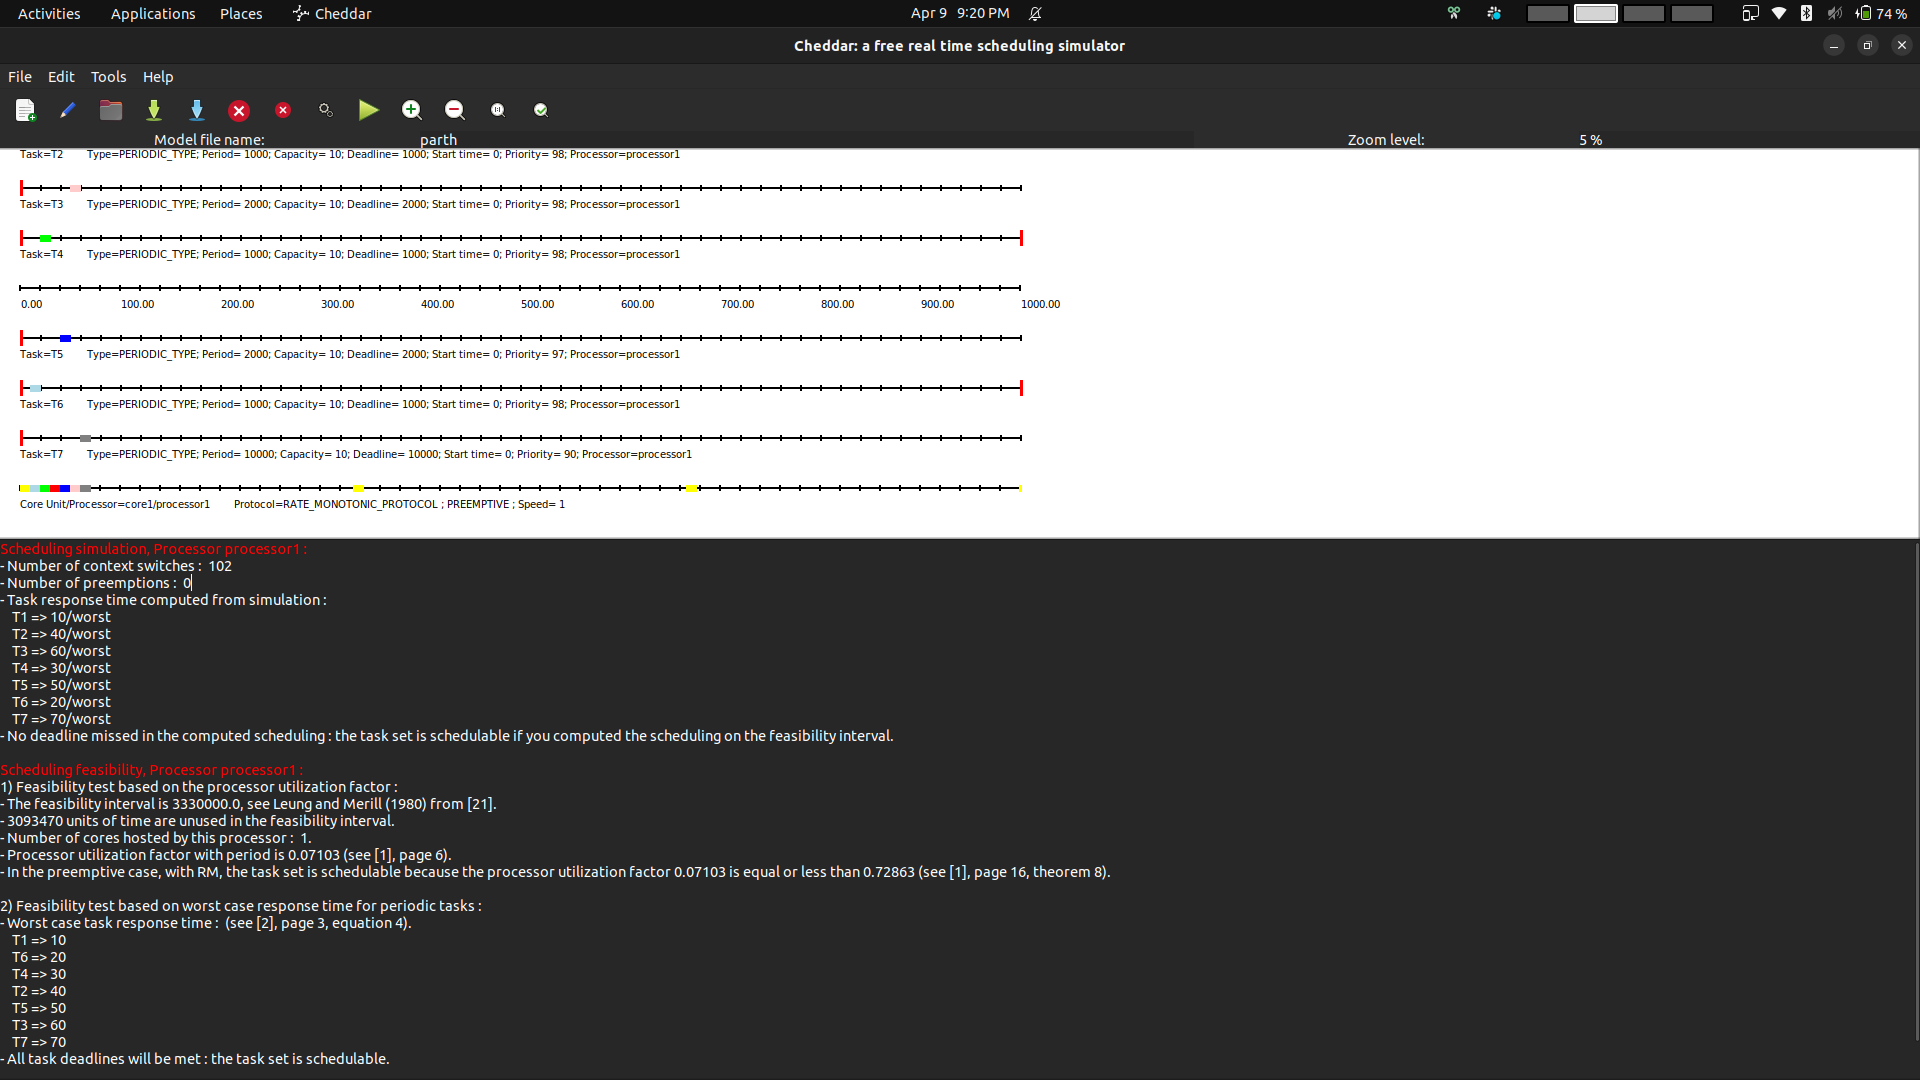
\includegraphics[scale=0.25]{figures/seqgen.png}
				\caption{Cheddar Analysis for seqgen (30Hz)}

			\end{figure}
			We can see that here the tasks are schedulable and feasibile, as the CPU utilization is very low, approximately 0.07 means 7\%,

			\begin{figure}[H]
				\centering
				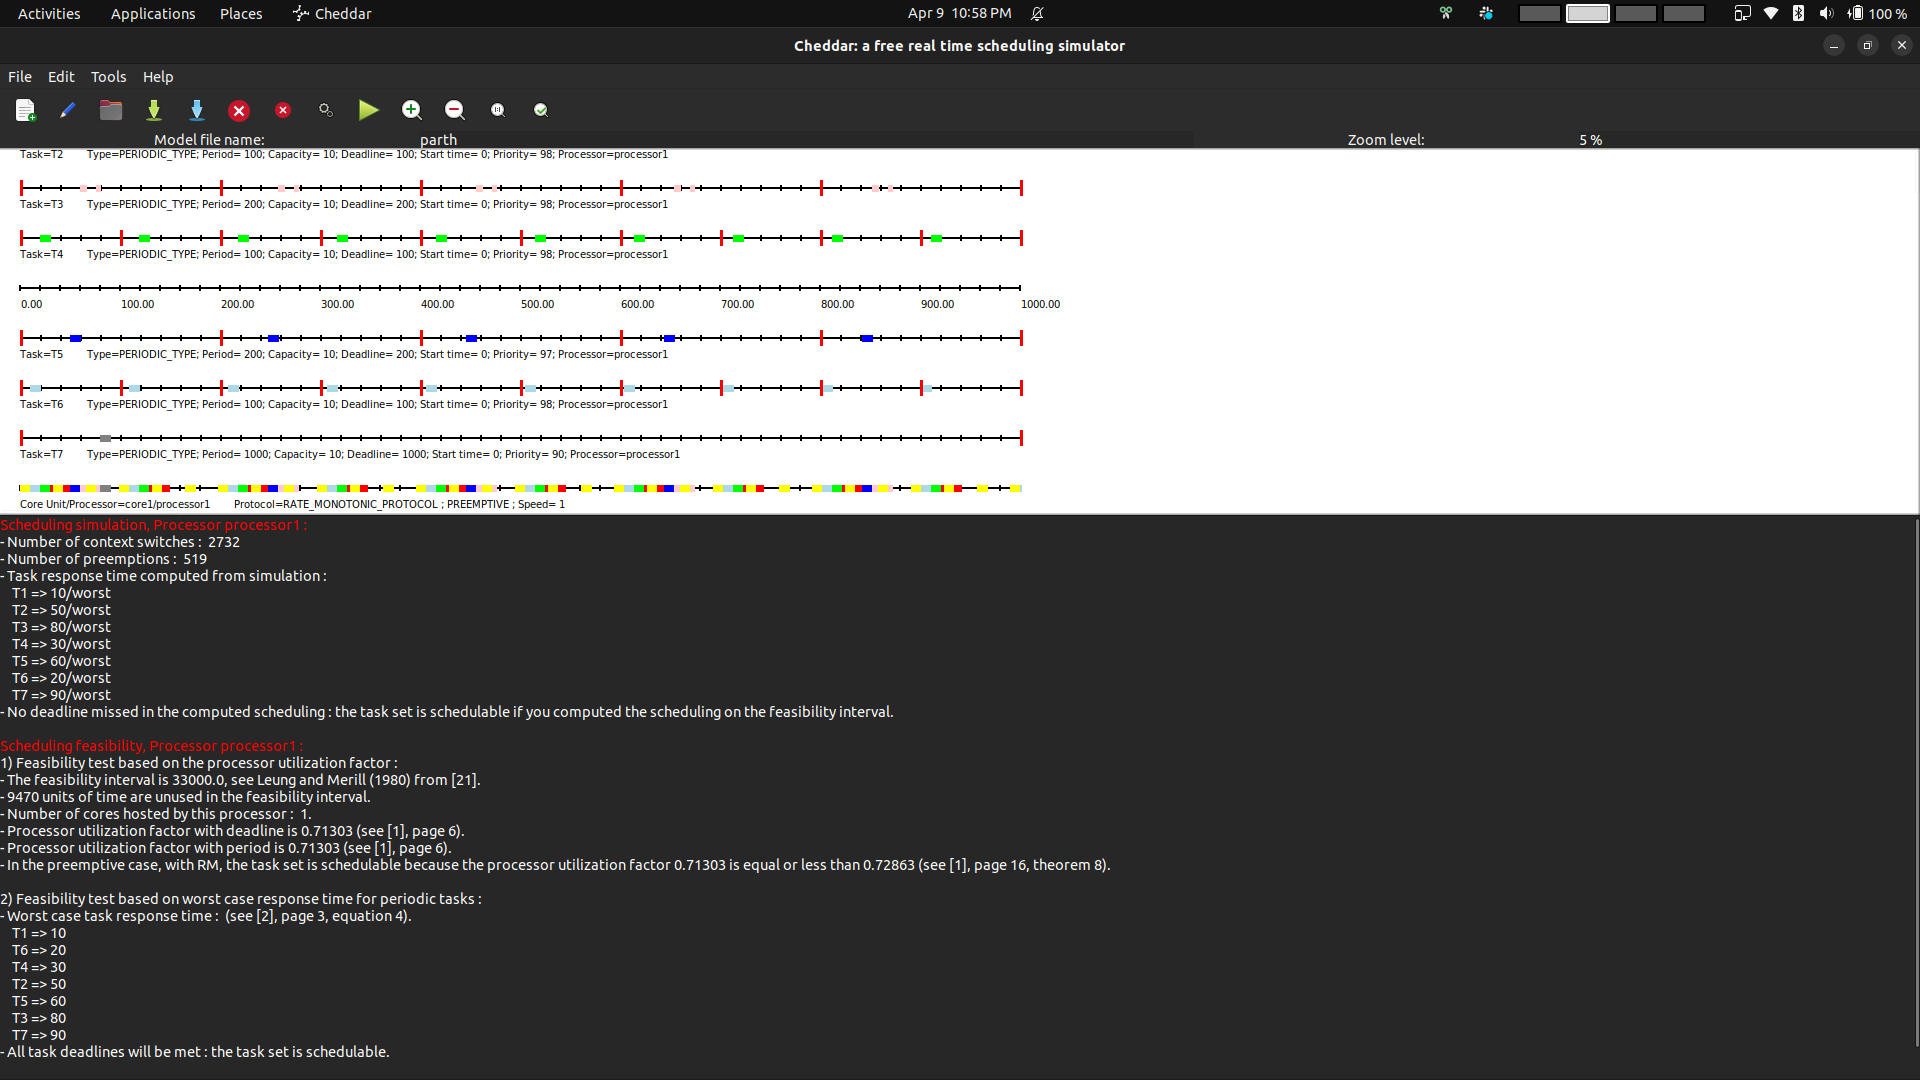
\includegraphics[scale=0.25]{figures/seqgen2x.png}
				\caption{Cheddar Analysis for seqgen2 (300Hz)}
			\end{figure}
			Here due to higher frequencies we can see that the CPU utilization is higher and we can see that the tasks are still schedulable.
			Utilization in this case is approximately 71.303\%.\\

			But in the both cases no deadline were missed and we could schedule those task that means tasks are schedulable.
			\subsection{Logs}
			\textbf{logs can be found in the answer\textgreater logs \textgreater q1\textgreater seqgen.txt and answer\textgreater logs\textgreater q1\textgreater seqgen2.txt}

	\end{enumerate}




	\section{Question 2}
	\begin{enumerate}
		\item[] \Q [30 points] Revise seqgen.c and seqgen2x.c to run under FreeRTOS on the DE1-SoC or
			TIVA board, by making each service a FreeRTOS task. Use the associated startup file in
			place of the existing startup file in FreeRTOS. Use an ISR driven by the PIT hardware timer
			to release each task at the given rate (you could even put the sequencer in the ISR). Build
			and execute the new code. Determine the worst case execution time (WCET) for each
			service by printing or logging timestamps between two points in your code or by use of a
			profiling tool. Determine D, T, and C for each service and create an RM schedule in
			Cheddar using your WCET estimates. Calculate the \% CPU utilization for this system.
			Compare this with the results you achieved under Linux in (1).
			\A
			\subsection{30 Hz sequencer}
			\textbf{Explanation of Sequencer:}

			\begin{enumerate}
				\item Interrupt Configuration:
				      \begin{itemize}
					      \item The sequencer ISR is triggered by a hardware timer, TIMER0, which is configured to generate periodic interrupts at a specified frequency (Hz).
					      \item The timer is set up using the TivaWare library functions, such as ROM\_SysCtlPeripheralEnable, ROM\_TimerConfigure, and ROM\_TimerLoadSet.
					      \item The ISR is registered with the timer using the TimerIntRegister function, specifying the ISR function (Timer0Isr\_Sequencer) to be called when the timer interrupt occurs.
				      \end{itemize}
				\item Interrupt Triggering:
				      \begin{itemize}
					      \item When the TIMER0 interrupt occurs, the processor suspends the currently executing task and jumps to the registered ISR, Timer0Isr\_Sequencer.
					      \item The ISR is executed in a special context, separate from the normal task execution, and has higher priority than regular tasks.
				      \end{itemize}
				\item Sequencer Functionality:
				      \begin{itemize}
					      \item The sequencer ISR keeps track of the number of cycles it has executed using the counter\_isr variable.
					      \item It uses the cycle count to determine which tasks should be released at each interval.
					      \item The ISR checks the cycle count against predefined constants to make release decisions. For example:
					            \begin{itemize}
						            \item Task 1 is released every 10 cycles (300 ms) when (counter\_isr \% 10) == 0.
						            \item Task 2, Task 4, and Task 6 are released every 30 cycles (990 ms) when (counter\_isr \% 30) == 0.
						            \item Task 3 and Task 5 are released every 60 cycles (1980 ms) when (counter\_isr \% 60) == 0.
						            \item Task 7 is released every 300 cycles (9900 ms) when (counter\_isr \% 300) == 0.
					            \end{itemize}
					      \item When a task needs to be released, the ISR gives the corresponding synchronization semaphore using the xSemaphoreGive function from FreeRTOS.
					      \item The released tasks are then scheduled by the FreeRTOS scheduler based on their priorities and the available system resources.
				      \end{itemize}
				\item Logging and Debugging:
				      \begin{itemize}
					      \item The sequencer ISR includes logging statements using the UARTprintf function to provide visibility into the system's behavior.
					      \item It logs the current cycle count and the corresponding sequencer cycle, allowing developers to track the progress of the sequencer and identify any anomalies or missed releases.
				      \end{itemize}
				\item Termination Condition:
				      \begin{itemize}
					      \item The sequencer ISR checks if the counter\_isr has exceeded a predefined limit (SEQUENCER\_COUNT).
					      \item When the limit is reached, the ISR performs the following actions:
					            \begin{itemize}
						            \item It releases all tasks one final time using their respective semaphores.
						            \item It sets the abort\_test flag to true, indicating that the system should terminate.
						            \item It disables the TIMER0 interrupt using the ROM\_TimerDisable function to prevent further interrupts.
					            \end{itemize}
				      \end{itemize}
			\end{enumerate}



			\textbf{output:}
			\begin{enumerate}
				\item Sequencer Thread Execution: The output begins with lines indicating the execution of the sequencer thread, which is triggered by the Timer0Isr\_Sequencer interrupt service routine (ISR). Each line follows the format:

				      \begin{lstlisting}[language=C]
Sequencer Thread ran at <timestamp> ms and Cycle of sequencer <cycle_count>
\end{lstlisting}
				      \begin{itemize}
					      \item The \textless timestamp \textgreater represents the current time in milliseconds since
					            the start of the system.

					      \item The \textless cycle\_count \textgreater represents the current cycle of the sequencer,
					            incremented each time the ISR is triggered.
				      \end{itemize}
				      For example:

				      \begin{lstlisting}[language=C]
Sequencer Thread ran at 33 ms and Cycle of sequencer 1
Sequencer Thread ran at 66 ms and Cycle of sequencer 2
...
\end{lstlisting}
				      These lines indicate that the sequencer thread is running periodically, with a cycle time of approximately 33 milliseconds. The cycle count increases by 1 each time the ISR is triggered.


				\item Task Execution: The output also includes lines indicating the execution of individual tasks. Each task line follows the format:
				      \begin{lstlisting}[language=C]
Task <task_number> (<task_name>) Start Time:<start_time> ms, 
	Release count <release_count>
Task <task_number> (<task_name>) Completion Time:<completion_time> ms, 
	Execution Time:<execution_time> ms
				\end{lstlisting}
				      \begin{itemize}
					      \item The \textless task\_number \textgreater represents the task identifier (e.g., Task 1, Task 2, etc.).
					      \item The \textless task\_name \textgreater represents the name of the task (e.g., Frame Sampler thread, Time-stamp with Image Analysis thread, etc.).
					      \item The \textless start\_time \textgreater represents the start time of the task in milliseconds since the start of the system.
					      \item The \textless release\_count \textgreater represents the number of times the task has been released by the sequencer.
					      \item The \textless completion\_time \textgreater represents the completion time of the task in milliseconds since the start of the system.
					      \item The \textless execution\_time \textgreater represents the execution time of the task in milliseconds, calculated as the difference between the completion time and the start time.
				      \end{itemize}

				\item Task Release Patterns: By analyzing the output, you can observe the release patterns of different tasks based on the sequencer cycle count. For example:
				      \begin{itemize}
					      \item Task 1 (Frame Sampler thread) is released every 10 cycles (approximately every 333 ms).
					      \item Task 2 (Time-stamp with Image Analysis thread), Task 4 (Time-stamp Image Save to File thread), and Task 6 (Send Time-stamped Image to Remote thread) are released every 30 cycles (approximately every 1000 ms).
					      \item Task 3 (Difference Image Proc thread) and Task 5 (Processed Image Save to File thread) are released every 60 cycles (approximately every 2000 ms).
					      \item Task 7 (10 sec Tick Debug thread) is released every 300 cycles (approximately every 10000 ms).
				      \end{itemize}
				      These release patterns align with the logic implemented in the sequencer ISR, where tasks are released based on the cycle count and their respective release intervals.
			\end{enumerate}




			\begin{lstlisting}[language=C]
***** Task 1 wcet 11 total_exectution_time 929 execution unit 90 *****

***** Task 2 wcet 11 total_exectution_time 309 execution unit 30 *****

***** Task 3 wcet 10 total_exectution_time 140 execution unit 14 *****

***** Task 4 wcet 10 total_exectution_time 300 execution unit 30 *****

***** Task 5 wcet 11 total_exectution_time 154 execution unit 14 *****

***** Task 6 wcet 10 total_exectution_time 290 execution unit 29 *****

***** Task 7 wcet 10 total_exectution_time 20 execution unit 2 *****
			\end{lstlisting}

			The output analysis provides a summary of the worst-case execution time, total execution time, and the number of times each task has been executed during the system's run. This information is valuable for understanding the timing behavior and resource utilization of each task.\\


			The output analysis provides a summary of the worst-case execution time, total execution time, and the number of times each task has been executed during the system's run. This information is valuable for understanding the timing behavior and resource utilization of each task.

			\begin{lstlisting}
Sequencer Thread ran at 999 ms and Cycle of sequencer 30
Task 1 (Frame Sampler thread) Start Time:1000 ms, Release count 3
Task 1 (Frame Sampler thread) Completion Time:1010 ms, Execution Time:10 ms
Task 2 (Time-stamp with Image Analysis thread) Start Time:1011 ms, Release count 1
Task 2 (Time-stamp with Image Analysis thread) 
Completion Time:1021 ms, Execution Time:10 ms

Task 4 (Time-stamp Image Save to File thread) Start Time:1022 ms, Release count 1
Task 4 (Time-stamp Image Save to File thread) 
CompSequencer Thread ran at 1033 ms and Cycle of sequencer 31

letion Time:1032 ms, Execution Timet:10 ms
Task 6 (Send Time-stamped Image to Remote thread) Start Time:1034 ms, Release count 1
Task 6 (Send Time-stamped Image to Remote thread)
Completion Time:1044 ms, Execution Time:10 ms
			\end{lstlisting}



			In this output, we can observe that multiple tasks are being released at the 30th cycle of the sequencer (999 ms). Let's break down the execution sequence:
			\begin{enumerate}
				\item Task 1 (Frame Sampler thread):\\
				      Released at 1000 ms with a release count of 3.\\
				      Starts executing immediately because it has the highest priority among the released tasks.\\
				      Completes execution at 1010 ms with an execution time of 10 ms.
				\item Task 2 (Time-stamp with Image Analysis thread):\\
				      Released at 1011 ms with a release count of 1.\\
				      Starts executing after Task 1 completes because it has the next highest priority.
				      Completes execution at 1021 ms with an execution time of 10 ms.\\
				\item Task 4 (Time-stamp Image Save to File thread):\\
				      Released at 1022 ms with a release count of 1.\\
				      Starts executing after Task 2 completes because it has the next highest priority.
				      Completes execution at 1032 ms with an execution time of 10 ms.\\
				\item Sequencer Thread:\\
				      Runs at 1033 ms, indicating the 31st cycle of the sequencer.\\
				\item Task 6 (Send Time-stamped Image to Remote thread):\\
				      Released at 1034 ms with a release count of 1.\\
				      Starts executing after the sequencer thread completes because it has the next highest priority among the remaining tasks.\\
				      Completes execution at 1044 ms with an execution time of 10 ms.
			\end{enumerate}




			In this scenario, with preemption disabled, the tasks are executed based on their priorities and release times. The task with the highest priority among the released tasks starts executing first, and it runs to completion before the next highest priority task begins execution.

			The execution sequence follows this pattern:
			\begin{enumerate}
				\item Task 1 (highest priority) executes and completes.
				\item Task 2 (next highest priority) executes and completes.
				\item Task 4 (next highest priority) executes and completes.
				      Sequencer Thread runs.
				\item Task 6 (remaining highest priority) executes and completes.
			\end{enumerate}

			The tasks with lower priorities wait for the higher priority tasks to complete before starting their execution. This non-preemptive behavior ensures that each task runs to completion without being interrupted by other tasks, even if they have higher priorities.\\


			In this scenario, all the threads are released simultaneously, but their execution order is determined by their assigned priorities. The task with the highest priority (Task 1) starts executing first and runs to completion. Then, the task with the next highest priority (Task 6) begins execution, followed by Task 2, Task 3, Task 5, and finally Task 7.

			The execution sequence follows the priority order:
			\begin{enumerate}
				\item Task 1 (highest priority)
				\item Task 6
				\item Task 2
				\item Task 3
				\item Task 5
				\item Task 7 (lowest priority)
			\end{enumerate}


			Each task runs to completion before the next task in the priority order starts executing. This behavior is consistent with the non-preemptive scheduling approach, where a task runs uninterrupted until it completes, even if higher priority tasks are released during its execution.\\


			Let's compare the worst-case execution time (WCET), jitter, predictability, determinism, and other important scheduling parameters between the FreeRTOS and POSIX implementations based on the provided output.\\

			Worst-Case Execution Time (WCET):\\
			\begin{enumerate}
				\item FreeRTOS:
				      \begin{itemize}
					      \item Task 1: 11 ms
					      \item Task 2: 11 ms
					      \item Task 3: 10 ms
					      \item Task 4: 10 ms
					      \item Task 5: 11 ms
					      \item Task 6: 10 ms
					      \item Task 7: 10 ms
				      \end{itemize}
				\item POSIX:
				      \begin{itemize}
					      \item Task 1: 92.489014 ms (set to 100ms)
					      \item Task 2: 85.020996 ms (set to 100ms)
					      \item Task 3: 90.000977 ms (set to 100ms)
					      \item Task 4: 86.266846 ms (set to 100ms)
					      \item Task 5: 88.769043 ms (set to 100ms)
					      \item Task 6: 177.165039 ms (set to 100ms)
					      \item Task 7: 168.037109 ms (set to 100ms)
				      \end{itemize}

			\end{enumerate}


			The WCET values for the POSIX implementation are significantly higher compared to the FreeRTOS implementation. This difference can be attributed to the overhead of the POSIX threading model and the impact of the Linux scheduler on task execution times.
			\textbf{Jitter:}
			\begin{enumerate}
				\item FreeRTOS: The jitter in the FreeRTOS implementation appears to be minimal, as the execution times are consistent across different instances of each task.
				\item POSIX: The POSIX implementation exhibits higher jitter, as evident from the variations in execution times for each task. For example, Task 6 has a WCET of 177.165039 ms, while its average execution time is 168.942459 ms, indicating significant jitter.
			\end{enumerate}

			\textbf{Predictability and Determinism:}
			\begin{enumerate}
				\item FreeRTOS: The FreeRTOS implementation demonstrates better predictability and determinism due to the consistent execution times and minimal jitter observed across task instances.
				\item POSIX: The POSIX implementation shows reduced predictability and determinism compared to FreeRTOS. The higher jitter and variable execution times make it more challenging to guarantee strict timing constraints.
			\end{enumerate}

			\textbf{Task Execution Units:}
			\begin{enumerate}
				\item FreeRTOS: The number of execution units for each task is consistent with the expected values based on the task periods and the total execution time.
				\item POSIX: The number of execution units for each task is also consistent with the expected values, indicating that the tasks are being released and executed according to their specified periods.
			\end{enumerate}

			\textbf{Scheduler Overhead:}
			\begin{enumerate}
				\item FreeRTOS: The FreeRTOS scheduler is designed for real-time embedded systems and has low overhead, contributing to the lower WCET values and minimal jitter observed.
				\item POSIX: The POSIX implementation, running on a Linux system, has higher scheduler overhead due to the complexities of the Linux scheduler and the need to manage multiple processes and threads. This overhead can impact the predictability and determinism of task execution.
			\end{enumerate}

			The differences in WCET, jitter, predictability, and determinism between the FreeRTOS and POSIX implementations can be attributed to several factors:

			\textbf{Real-Time Operating System (RTOS) vs. General-Purpose Operating System (GPOS):}
			\begin{enumerate}
				\item FreeRTOS is a real-time operating system specifically designed for embedded systems, with a focus on determinism and real-time performance.
				\item POSIX, in this case running on Linux, is a general-purpose operating system that prioritizes overall system performance and fairness rather than strict real-time guarantees.
			\end{enumerate}

			\textbf{Scheduler Design:}
			\begin{enumerate}
				\item FreeRTOS has a simple and efficient scheduler tailored for real-time tasks, with minimal overhead and deterministic behavior.
				\item The Linux scheduler, used in the POSIX implementation, is more complex and designed to handle a wide range of workloads, which can introduce additional overhead and variability in task execution times.
			\end{enumerate}

			\textbf{System Overhead:}
			\begin{enumerate}
				\item FreeRTOS, being a lightweight RTOS, has lower system overhead compared to Linux, which runs multiple processes and services in the background.
				\item The higher system overhead in Linux can interfere with the execution of real-time tasks and contribute to increased jitter and reduced predictability.
			\end{enumerate}

			\subsubsection{C, D, T}
			\begin{table}[H]
				\centering
				\begin{tabular}{l c c c c}
					\hline
					\textbf{Service} & \textbf{Service	Deadline (D)} & \textbf{Computation Time (C)} & \textbf{Period (T)} & \textbf{WCET} \\\hline
					                 &                              &                                                                     \\
					Service\_1       & 333 ms                      & 10 ms                         & 333 ms              & 13.337891 ms  \\
					Service\_2       & 1000 ms                       & 10 ms                         & 1000 ms             & 12.876953 ms  \\
					Service\_3       & 2000 ms                       & 10 ms                         & 2000 ms             & 25.176025 ms  \\
					Service\_4       & 1000 ms                       & 10 ms                         & 1000 ms             & 25.923828 ms  \\
					Service\_5       & 2000 ms                       & 10 ms                         & 2000 ms             & 24.409912 ms  \\
					Service\_6       & 1000 ms                       & 10 ms                         & 1000 ms             & 26.864014 ms  \\
					Service\_7       & 10000 ms                      & 10 ms                         & 1000 ms             & 68.493164 ms  \\

					\hline\hline
				\end{tabular}
				\caption{C, T, D, for 10ms load, and sequencer frequency set to 30Hz in POSIX}
			\end{table}

			\begin{table}[H]
				\centering
				\begin{tabular}{l c c c c}
					\hline
					\textbf{Service} & \textbf{Service	Deadline (D)} & \textbf{Computation Time (C)} & \textbf{Period (T)} & \textbf{WCET} \\\hline
					                 &                              &                                                                     \\
					Service\_1       & 333 ms                      & 100 ms                         & 333 ms              & 97 ms  \\
					Service\_2       & 1000 ms                       & 100 ms                         & 1000 ms             & 97 ms  \\
					Service\_3       & 2000 ms                       & 100 ms                         & 2000 ms             & 97 ms  \\
					Service\_4       & 1000 ms                       & 100 ms                         & 1000 ms             & 97 ms  \\
					Service\_5       & 2000 ms                       & 100 ms                         & 2000 ms             & 97 ms  \\
					Service\_6       & 1000 ms                       & 100 ms                         & 1000 ms             & 96 ms  \\
					Service\_7       & 10000 ms                      & 10 ms                         & 1000 ms             & 96 ms  \\

					\hline\hline
				\end{tabular}
				\caption{C, T, D, for 100ms load, and sequencer frequency set to 30Hz in freeRTOS}
			\end{table}

			\subsubsection{Cheddar}

			\subsection{TIVA freeRTOS similar to seqgen2x(300Hz)}

			\textbf{Output}
			\begin{lstlisting}
***** Task 1 wcet 13 total_exectution_time 1072 execution unit 90 *****

***** Task 2 wcet 13 total_exectution_time 351 execution unit 29 *****

***** Task 3 wcet 13 total_exectution_time 176 execution unit 14 *****

***** Task 4 wcet 13 total_exectution_time 361 execution unit 29 *****

***** Task 5 wcet 12 total_exectution_time 168 execution unit 14 *****

***** Task 6 wcet 12 total_exectution_time 345 execution unit 29 *****

***** Task 7 wcet 12 total_exectution_time 24 execution unit 2 *****
			\end{lstlisting}


			Here we can see that the load is set to again 10ms and we can see the similar behaviour in the output that this is more deterministic than the LINUX posix api, we are getting around +2 to 3 ms of jitter which is better than the Linux

			Note that we have set sequencer frequency to 300Hz and increased all the frequencies by multiplier of 10.

			\subsubsection{C, T, D}
			\begin{table}[H]
				\centering
				\begin{tabular}{l c c c c}
					\hline
					\textbf{Service} & \textbf{Service	Deadline (D)} & \textbf{Computation Time (C)} & \textbf{Period (T)} & \textbf{WCET} \\\hline
					                 &                              &                                                                     \\
					Service\_1       & 33.3 ms                      & 10 ms                         & 333 ms              & 13.337891 ms  \\
					Service\_2       & 100 ms                       & 10 ms                         & 1000 ms             & 12.876953 ms  \\
					Service\_3       & 200 ms                       & 10 ms                         & 2000 ms             & 25.176025 ms  \\
					Service\_4       & 100 ms                       & 10 ms                         & 1000 ms             & 25.923828 ms  \\
					Service\_5       & 200 ms                       & 10 ms                         & 2000 ms             & 24.409912 ms  \\
					Service\_6       & 100 ms                       & 10 ms                         & 1000 ms             & 26.864014 ms  \\
					Service\_7       & 1000 ms                      & 10 ms                         & 1000 ms             & 68.493164 ms  \\

					\hline\hline
				\end{tabular}
				\caption{C, T, D, for 10ms load, and sequencer frequency set to 30Hz}
			\end{table}

			\subsubsection{Cheddar}

			\begin{figure}[H]
				\centering
				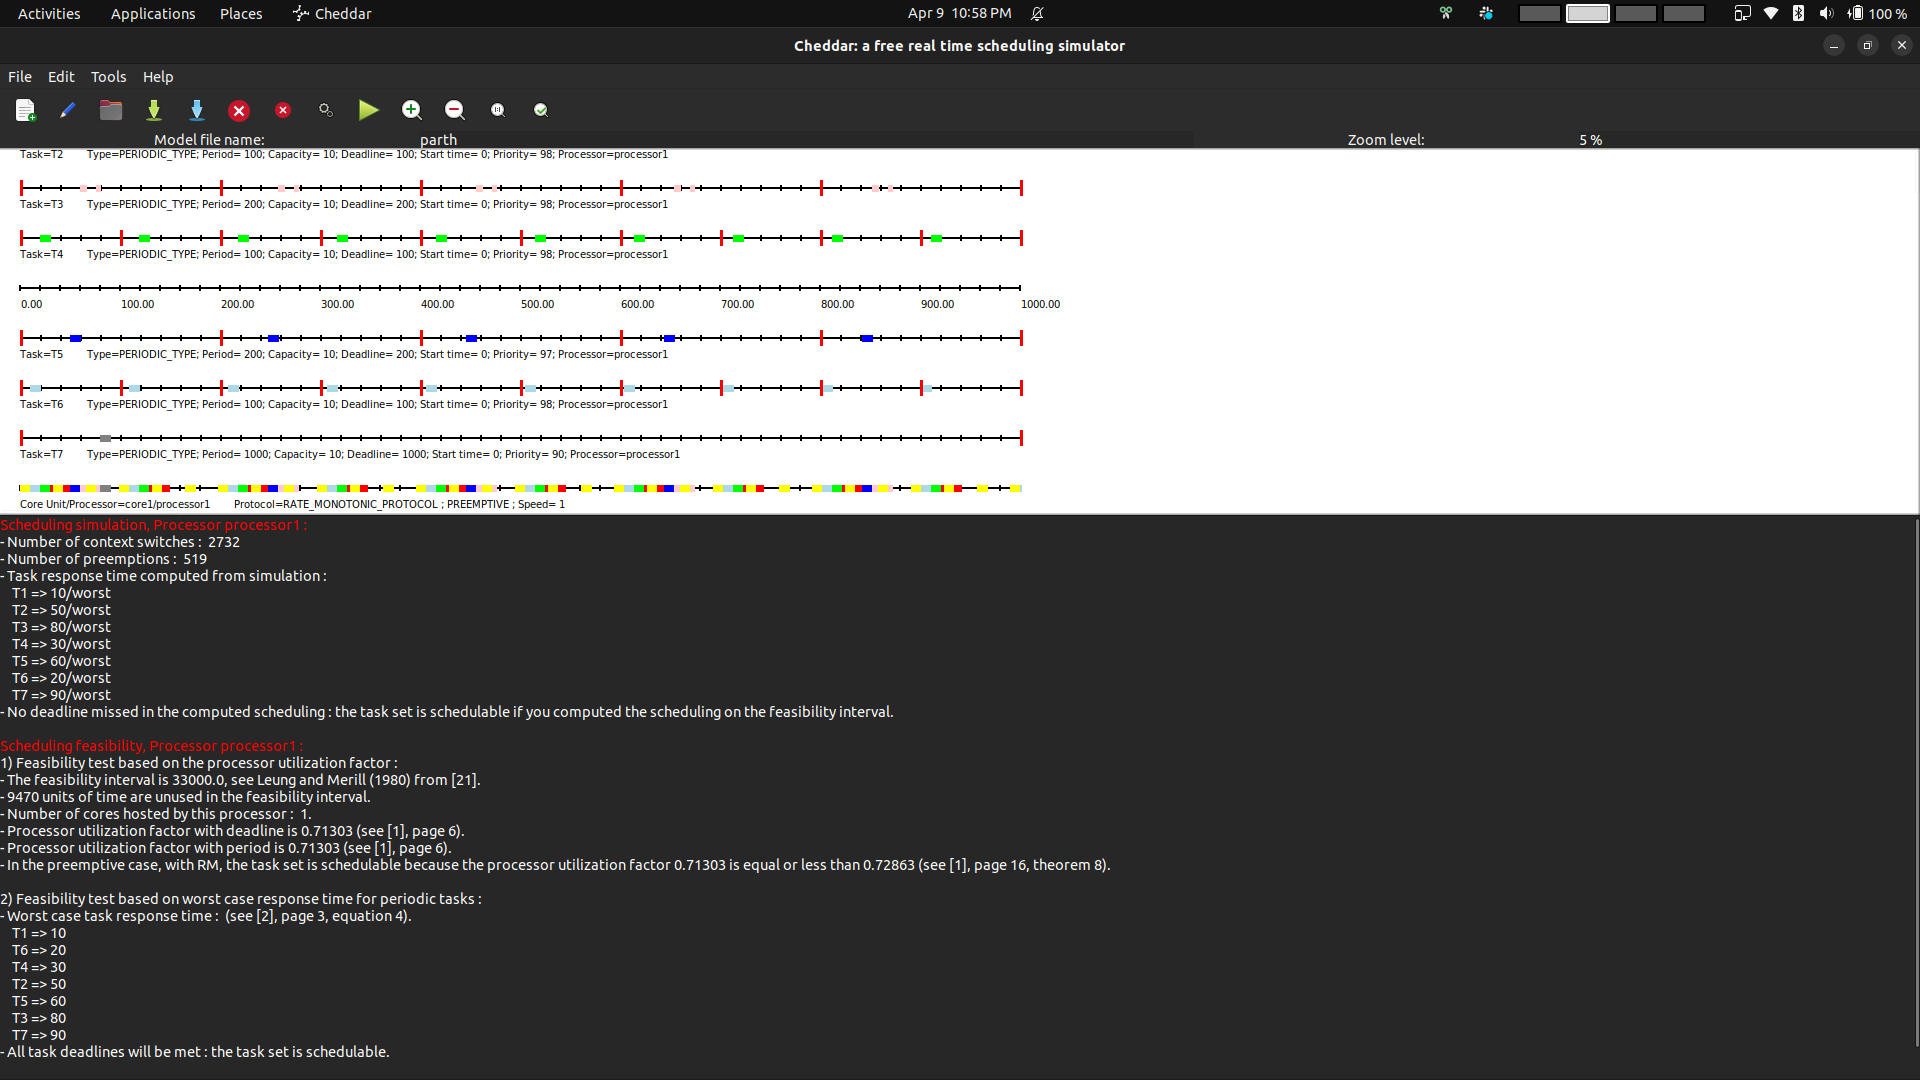
\includegraphics[scale=0.25]{figures/seqgen2x.png}
				\caption{Cheddar Analysis for seqgen2 (300Hz)}
			\end{figure}

			\subsection{Logs}

			\textbf{logs can be found in the answer\textgreater logs\textgreater q2\textgreater seqgen.txt and answer\textgreater logs\textgreater q2\textgreater seqgen2.txt}\\
			\textbf{Code can be found in the answer\textgreater code\textgreater q2\textgreater seqgen.c and answer\textgreater code\textgreater q2\textgreater seqgen2.c}

	\end{enumerate}




	\section{Question 3}
	\begin{enumerate}
		\item[] \Q [40 points] Revise seqgen.c from both previous systems to increase the sequencer frequency
			and all service frequencies by a factor of 100 (3000 Hz). Build and execute the code under
			Linux and FreeRTOS on your target boards as before. For both operating systems determine
			the worst case execution time (WCET) for each service by printing or logging timestamps
			between two points in your code or by use of a profiling tool. Determine D, T, and C for
			each service and create an RM schedule in Cheddar using your WCET estimates. Calculatethe \% CPU utilization for these systems. Compare results between Linux and FreeRTOS in
			this higher-speed case.
			\A

	\end{enumerate}

	\pagebreak

	Code is same as the TivaWare freeRTOS code for seqgen just the logs are removed as it was taking some time and changed the multiple value to 1000.\\

	In the provided output analysis, the multiplier has been increased to 100, meaning that all the services are running at 100 times their original frequency. Additionally, the execution time of each task has been reduced to 1 ms, and the UART printfs have been removed to minimize interference with task execution. Let's analyze the output in detail:

	Increasing the frequency of the services can have several effects on the system:
	\begin{itemize}
		\item Higher CPU utilization: With tasks executing more frequently, the CPU utilization will increase as more time is spent executing the tasks.
		\item Increased context switching: As tasks are released and executed more often, there will be more context switches between tasks, which can introduce overhead and affect overall system performance.
		\item Potential resource contention: If tasks compete for shared resources (e.g., memory, I/O devices), the increased frequency of execution may lead to more resource contention and potential delays or blocking.
		\item Timing constraints: The system must ensure that the increased frequency of task execution does not violate any timing constraints or deadlines associated with the tasks.
	\end{itemize}


	System Behavior:
	\begin{enumerate}
		\item The increased frequency and reduced execution time of tasks result in a more fine-grained and responsive system.
		\item The tasks are executed more frequently, allowing for faster processing and reaction to events.
		\item However, the higher frequency also leads to increased context switching and potential resource contention, which may impact the overall system performance. and cause of that we needed to remove extra logs and keep the interference as low as possible.
	\end{enumerate}


	The execution sequence follows the priority order:
	\begin{enumerate}
		\item Task 1 (highest priority)
		\item Task 6
		\item Task 2
		\item Task 3
		\item Task 5
		\item Task 7 (lowest priority)
	\end{enumerate}


	Each task runs to completion before the next task in the priority order starts executing. This behavior is consistent with the non-preemptive scheduling approach, where a task runs uninterrupted until it completes, even if higher priority tasks are released during its execution.\\
	\subsection{output}
	\begin{lstlisting}
				
***** Task 1 wcet 2 total_exectution_time 9040 execution unit 9000 *****

***** Task 2 wcet 1 total_exectution_time 2999 execution unit 2999 *****

***** Task 3 wcet 1 total_exectution_time 1499 execution unit 1499 *****

***** Task 4 wcet 2 total_exectution_time 4802 execution unit 2999 *****

***** Task 5 wcet 1 total_exectution_time 1499 execution unit 1499 *****

***** Task 6 wcet 2 total_exectution_time 3272 execution unit 2999 *****

***** Task 7 wcet 1 total_exectution_time 299 execution unit 299 *****

			\end{lstlisting}
	Let's compare the worst-case execution time (WCET), jitter, predictability, determinism, and other important scheduling parameters between the FreeRTOS and POSIX implementations based on the provided output.\\

	Worst-Case Execution Time (WCET):\\
	\begin{enumerate}
		\item FreeRTOS:
		      \begin{itemize}
			      \item Task 1: 2 ms
			      \item Task 2: 1 ms
			      \item Task 3: 1 ms
			      \item Task 4: 2 ms
			      \item Task 5: 1 ms
			      \item Task 6: 2 ms
			      \item Task 7: 1 ms
		      \end{itemize}
	\end{enumerate}

	\subsubsection{C, T, D}
			\begin{table}[H]
				\centering
				\begin{tabular}{l c c c c}
					\hline
					\textbf{Service} & \textbf{Service	Deadline (D)} & \textbf{Computation Time (C)} & \textbf{Period (T)} & \textbf{WCET} \\\hline
					                 &                              &                                                                     \\
					Service\_1       & 3.33 ms                      & 1 ms                         & 33 ms              & 2 ms  \\
					Service\_2       & 10 ms                       & 1 ms                         & 100 ms             & 1 ms  \\
					Service\_3       & 20 ms                       & 1 ms                         & 200 ms             & 1 ms  \\
					Service\_4       & 10 ms                       & 1 ms                         & 100 ms             & 2 ms  \\
					Service\_5       & 20 ms                       & 1 ms                         & 200 ms             & 1 ms  \\
					Service\_6       & 10 ms                       & 1 ms                         & 100 ms             & 2 ms  \\
					Service\_7       & 100 ms                      & 1 ms                         & 100 ms             & 1 ms  \\

					\hline\hline
				\end{tabular}
				\caption{C, T, D, for 10ms load, and sequencer frequency set to 3000Hz}
			\end{table}


			\begin{table}[H]
				\centering
				\begin{tabular}{l c c c c}
					\hline
					\textbf{Service} & \textbf{Service	Deadline (D)} & \textbf{Computation Time (C)} & \textbf{Period (T)} & \textbf{WCET} \\\hline
					                 &                              &                                                                     \\
					Service\_1       & 3.3 ms                      & 1 ms                         & 3.3 ms              & 1.700195  \\
					Service\_2       & 10 ms                       & 1 ms                         & 10 ms             & 1.650146  \\
					Service\_3       & 20 ms                       & 1 ms                         & 20 ms             & 3.070801 ms  \\
					Service\_4       & 10 ms                       & 1 ms                         & 10 ms             & 3.210938 ms  \\
					Service\_5       & 20 ms                       & 1 ms                         & 20 ms             & 10.370117 ms  \\
					Service\_6       & 10 ms                       & 1 ms                         & 10 ms             & 2.578125 ms  \\
					Service\_7       & 100 ms                      & 1 ms                         & 10 ms             & 10.051025 ms  \\

					\hline\hline
				\end{tabular}
				\caption{C, T, D, for 1ms load in POSIX}
			\end{table}
			Why is this happening ?? we have service one running at 3.33 ms and it has highest priority, service 2 and 6 has next highest priorities and we are releasing Task 2 first so Task 6 will run after task 2 and might get preempted by task 1. so WCET of T6 > WCET T2 and Tasks 3,4,5 Has next highest priorities so It can be preempted by Task 1,2 and so their worst case execution time is more. And finally Service 7 It might and might note get preempted by Task 1 as the probability of getting preempted by task 7 is less (it runs every 100ms) but in our case it is getting preempted as we are running the code 180000 times. This explains the output.

			\subsubsection{Cheddar}

			\begin{figure}[H]
				\centering
				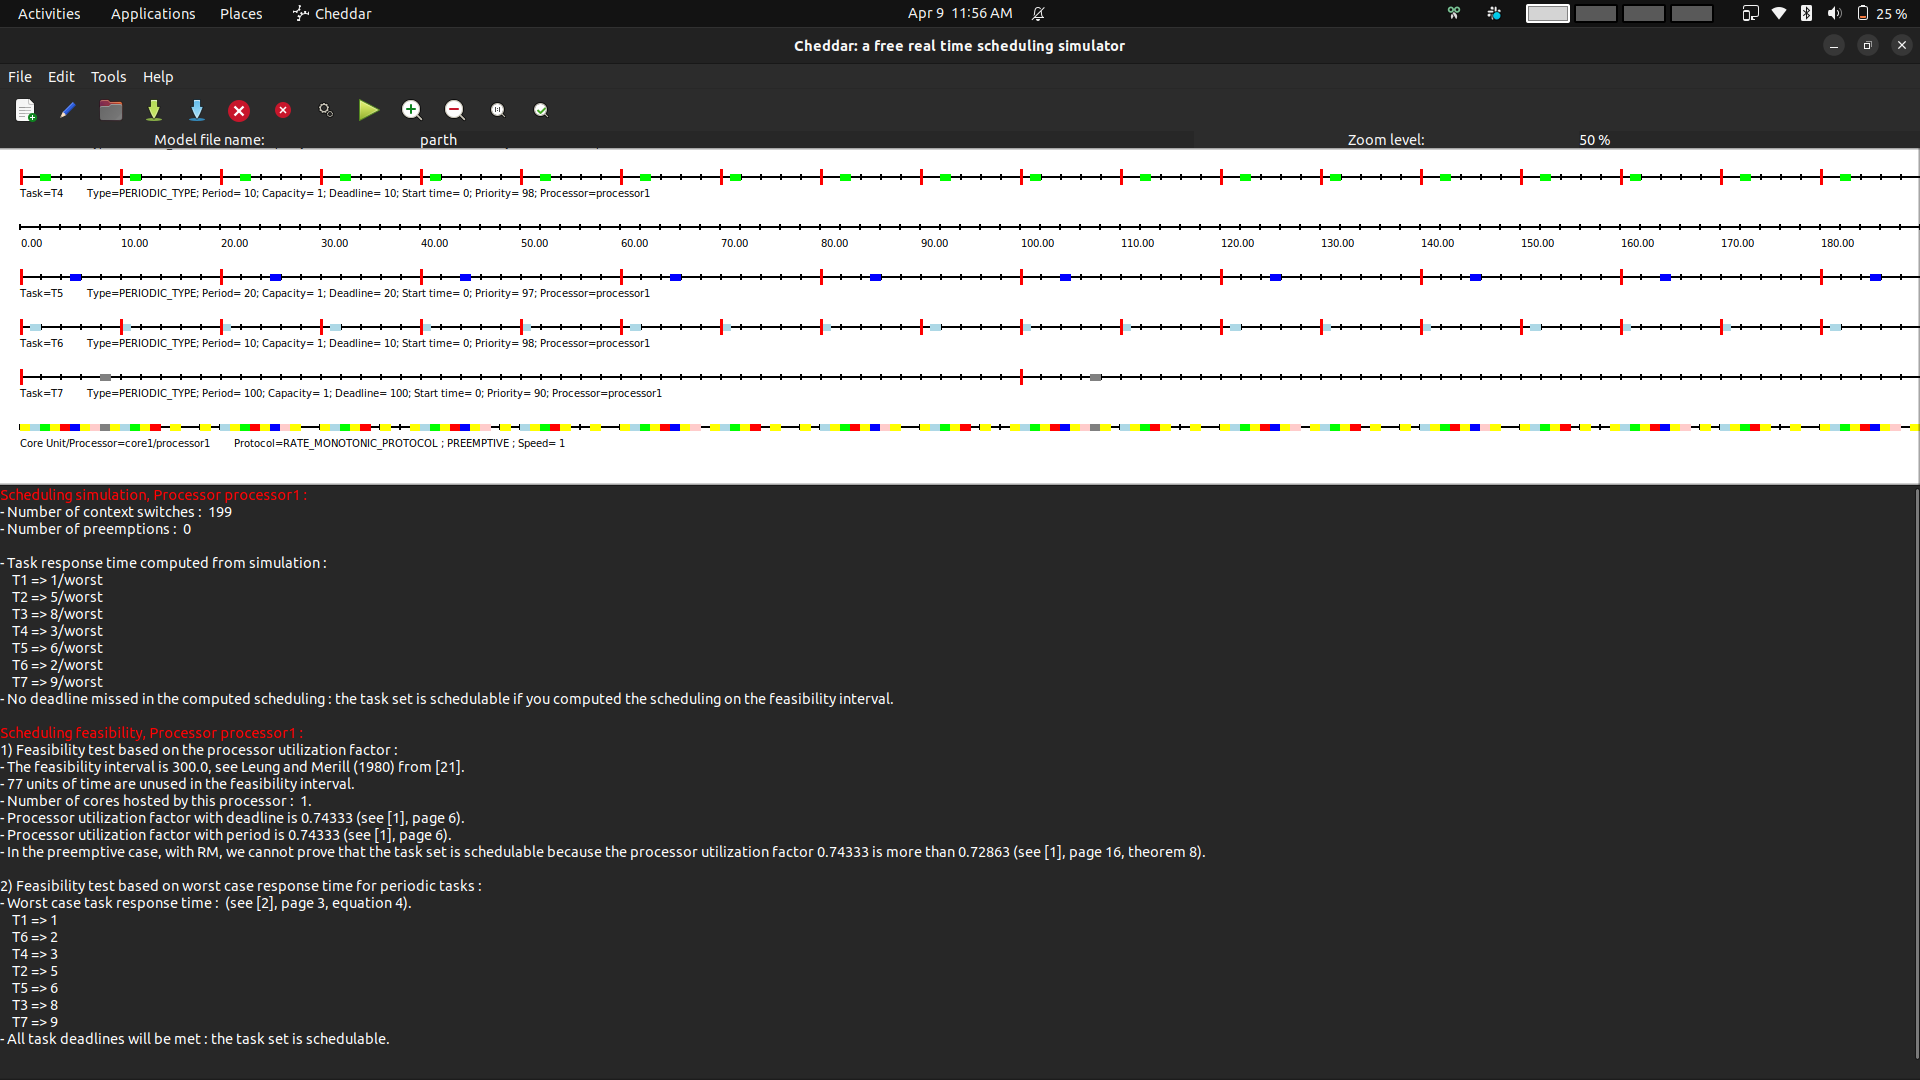
\includegraphics[scale=0.25]{figures/seqgen3000Hz.png}
				\caption{Cheddar Analysis for seqgen (30000Hz)}

			\end{figure}

			The processor utilization factor is calculated as 0.74333, which is more than the Liu \& Layland bound of 0.72863 for the preemptive case.\\
Since the utilization factor exceeds the bound, the simulator cannot prove that the task set is schedulable using this test. but since all the deadlines are met we can say that the tasks are feasible and schedulable.\\
			\subsection{conclusion}

			For high frequency cases, we saw that the TIVA board gave more predictable results compared to the Jetson board. Even though the TIVA board's update rate was set to a slower 1ms, it performed better than the Jetson board. The Jetson board has multiple cores and a higher clock speed. FreeRTOS is lightweight and ideal for real-time applications. It works better than Linux, which is meant for desktop applications. Using a real-time patch for Linux could improve its predictability. However, Linux runs background processes that may affect the application's predictability. There are many factors to consider when designing a hard real-time system. In conclusion, for higher frequencies, FreeRTOS proves to be more predictable than Linux.




			\subsection{Logs}

			\textbf{logs can be found in the answer\textgreater logs\textgreater q3\textgreater seqgen.txt}\\
			\textbf{Code can be found in the answer\textgreater code\textgreater q3\textgreater seqgen.c}


	\section{References}
	\begin{enumerate}
		\item ECEN 5623 Lecture slides material and example codes.
		\item REAL-TIME EMBEDDED COMPONENTS AND SYSTEMS with LINUX and RTOS, Sam Siewert John
		      Pratt (Chapter 6, 7 \& 8).
		\item Exercise 5 requirements included links and documentation.
	\end{enumerate}


\end{qanda}




\vfill
\hrule
\vspace{0.5cm}
\pagebreak
\begin{appendices}
	\section{C Code for the Implementation}
	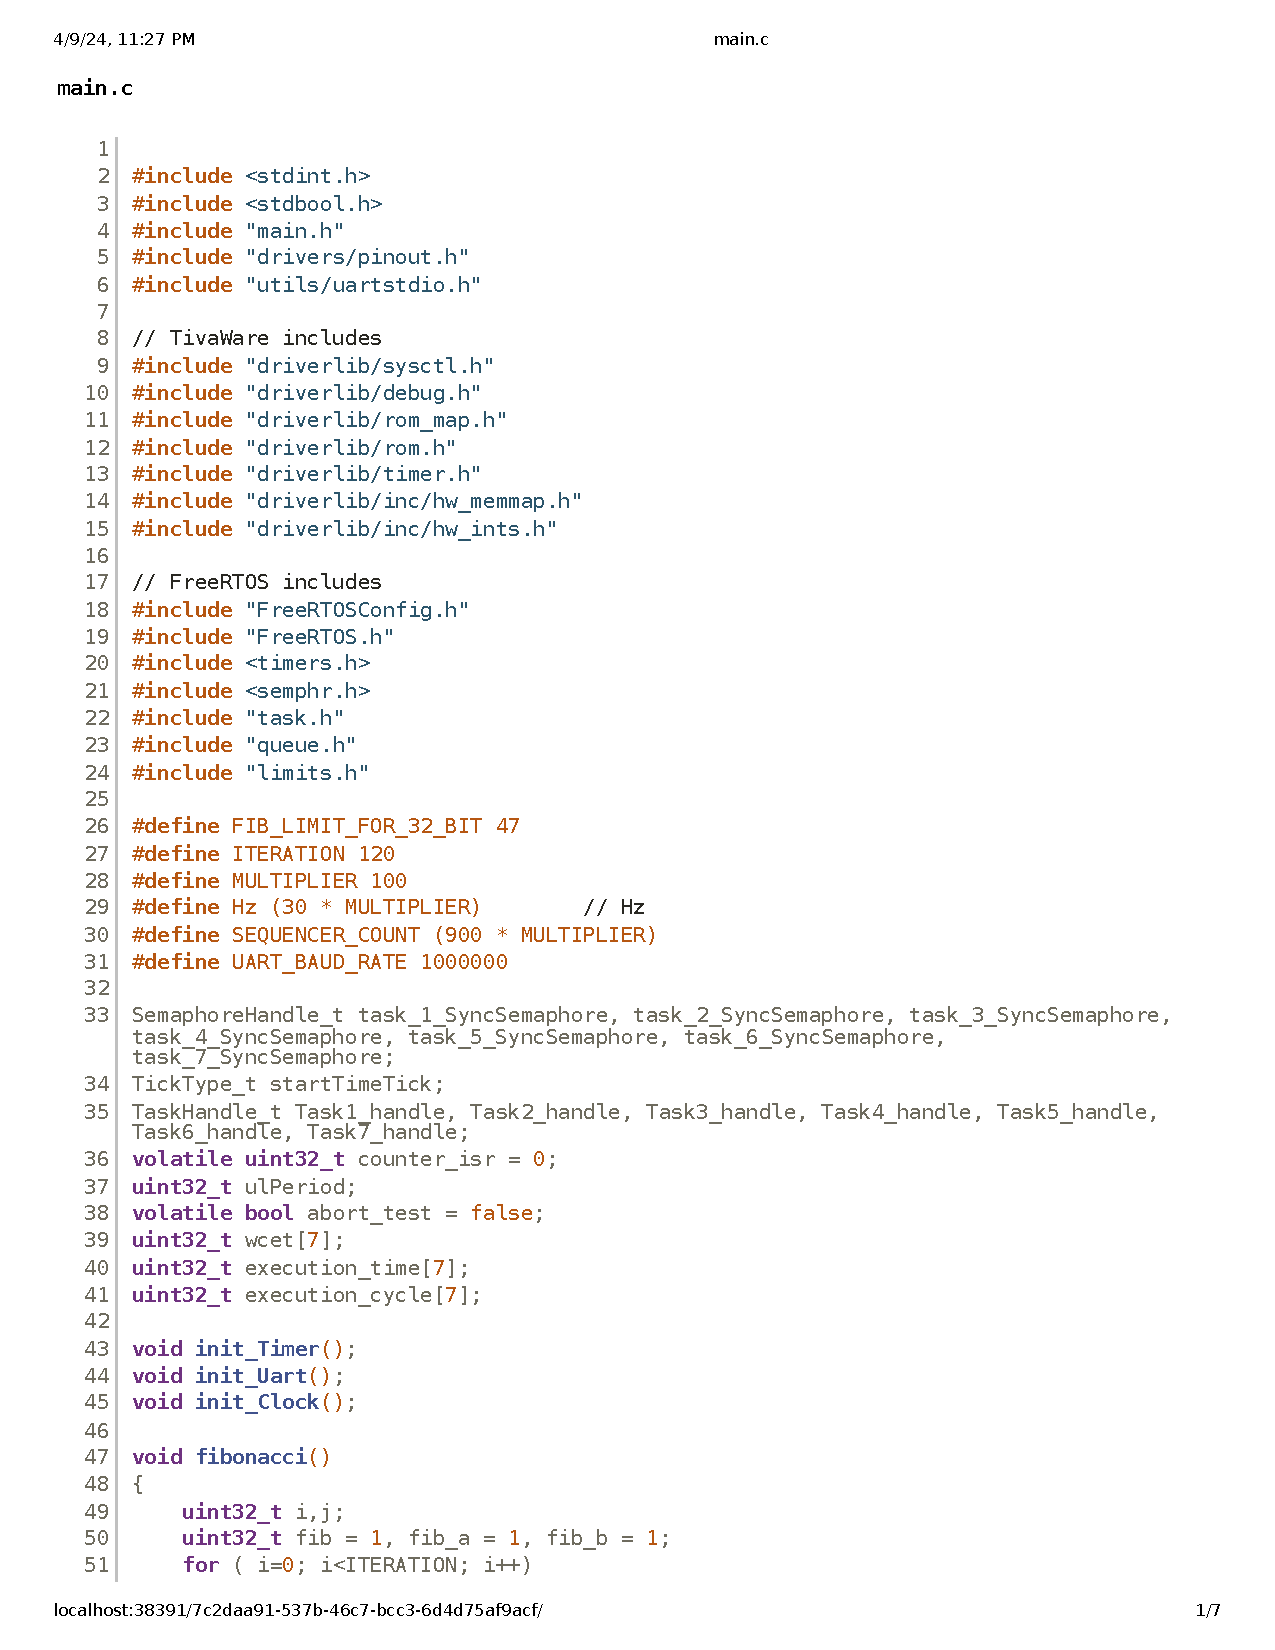
\includepdf[pages=-]{code/3000Hz.pdf}
	\pagebreak
	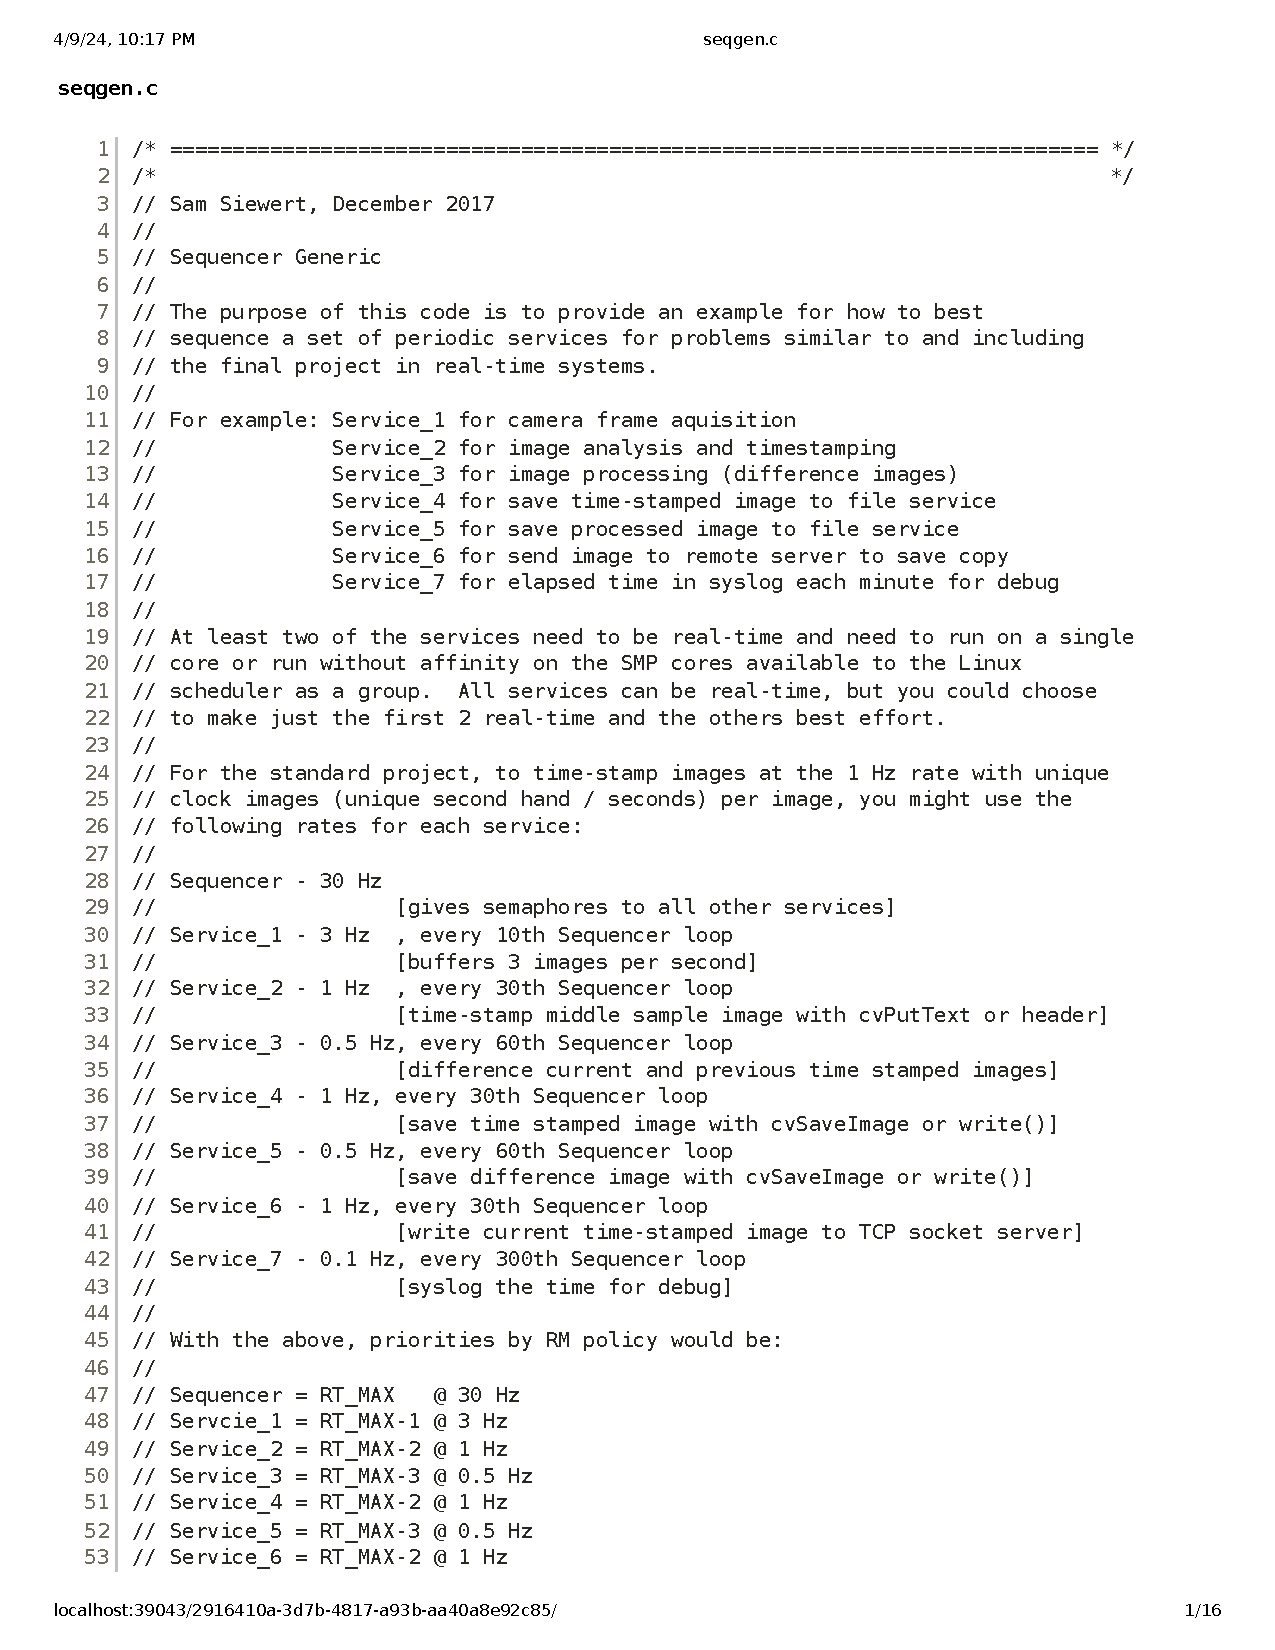
\includepdf[pages=-]{code/seqgen.c.pdf}
	\pagebreak
	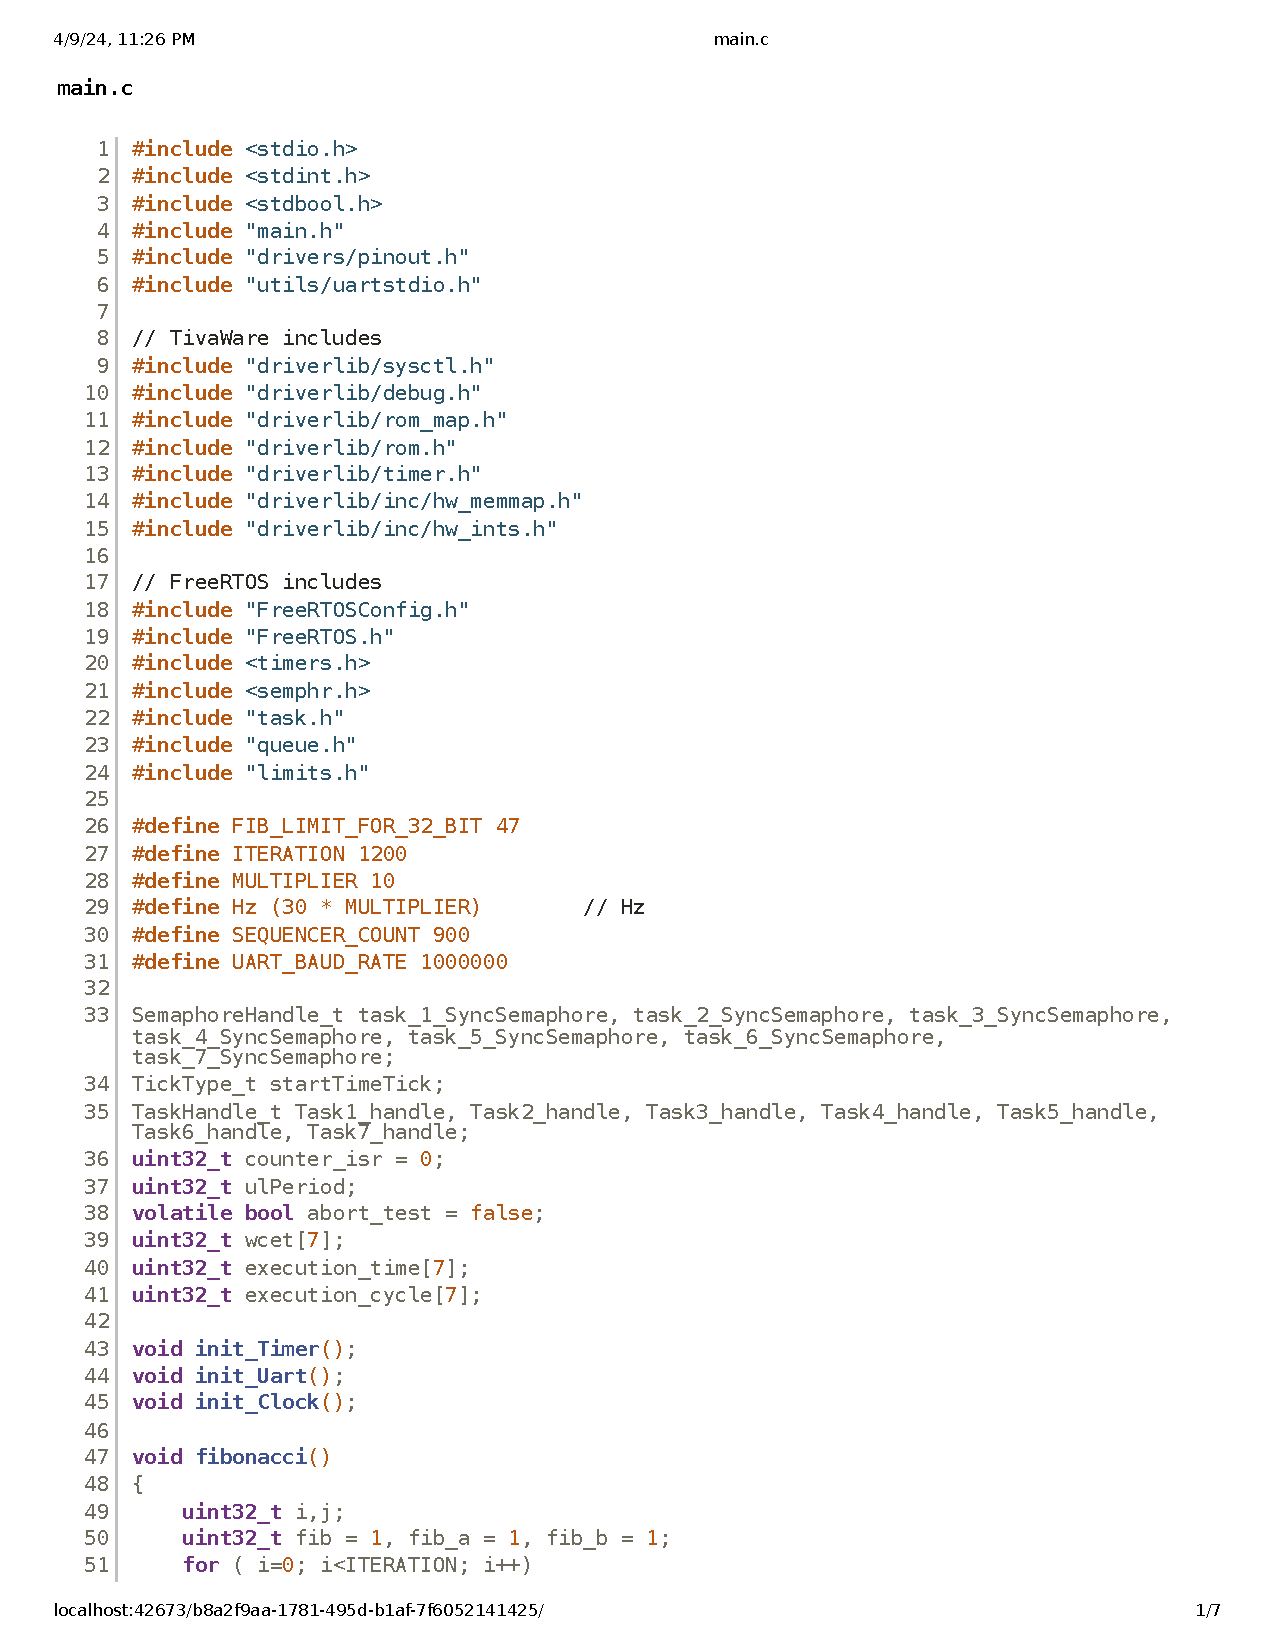
\includepdf[pages=-]{code/sequancer.pdf}
\end{appendices}


\vspace{1cm}
\hrule
\vspace{0.5cm}


%---------------------------------------------------------------------------
\end{document}
-
